\documentclass{article}

\usepackage[preprint]{corl_2026}

\usepackage[utf8]{inputenc}
\usepackage[T1]{fontenc}
\usepackage{amsmath,amssymb,bm}
\usepackage{booktabs}
\usepackage{array}
\usepackage{graphicx}
\usepackage{tikz}
\usetikzlibrary{arrows.meta,positioning,calc,fit,backgrounds}
\usepackage{listings}
\usepackage{xcolor}
\usepackage{microtype}
\usepackage{enumitem}

% ---------- notation ----------
\newcommand{\R}{\mathbb{R}}
\newcommand{\E}{\mathbb{E}}
\newcommand{\Tf}[2]{T^{#1}_{#2}}
\newcommand{\w}{\mathrm{w}}
\newcommand{\obj}{\mathrm{obj}}
\newcommand{\grip}{\mathrm{grip}}
\newcommand{\base}{\mathrm{b}}
\newcommand{\tgt}{\mathrm{target}}
\newcommand{\code}[1]{\texttt{#1}}
\newcommand{\subl}[1]{{\scriptsize\color{black!60}#1}}
\newcommand{\clamp}{\operatorname{clamp}}

% ---------- colours used in figures ----------
\definecolor{accent}{HTML}{1E6B86}
\definecolor{accentsoft}{HTML}{E2EEF2}
\definecolor{warnsoft}{HTML}{F6ECDC}
\definecolor{warn}{HTML}{8A5A12}
\definecolor{codebg}{HTML}{F4F5F4}

\lstset{
  basicstyle=\ttfamily\scriptsize,
  commentstyle=\color{black!55}\itshape,
  keywordstyle=\bfseries,
  backgroundcolor=\color{codebg},
  frame=single, framerule=0pt, framesep=4pt,
  columns=fullflexible, keepspaces=true,
  breaklines=true, showstringspaces=false,
  xleftmargin=4pt, xrightmargin=4pt,
}

\tikzset{
  blk/.style={draw, rounded corners=2pt, minimum height=8mm, minimum width=18mm, align=center, font=\small, inner sep=3pt},
  key/.style={draw=accent, thick},
  sub/.style={font=\scriptsize\color{black!60}},
  arr/.style={-{Latex[length=2mm]}, thick},
  karr/.style={-{Latex[length=2mm]}, thick, accent},
  darr/.style={-{Latex[length=2mm]}, thick, dashed},
}

\title{Discovering Where Episodes Begin:\\ How OmniReset Generates Its Reset-State Datasets}

\author{
  Tri Wahyu Guntara\\
  Tutorial notes on the UWLab OmniReset code base\\
}

\begin{document}
\maketitle

\begin{abstract}
A reinforcement-learning policy for peg insertion can only become competent in the situations it has been placed in. OmniReset therefore begins each training episode from a library of \emph{reset states}, complete snapshots of the scene that physics has already accepted as stable, organised into four families: the object anywhere with the hand anywhere, the object resting with the hand grasping it, the object held in the air, and the object partly inserted with the hand on it. This tutorial explains how that library is produced. We define what a reset state is and how it is stored, describe the two auxiliary datasets of grasps and partial assemblies on which the grasped families depend, walk through one recording attempt from the reset events to the export decision, derive the inverse-kinematics placement of the hand on a sampled grasp, and examine the success test clause by clause. We close with the commands that run the generator, the failure modes that motivated each clause, and exercises for the reader. Every statement is tied to the implementation on the \code{feature/forge-omnireset} branch.
\end{abstract}

\keywords{Reset-state distributions, Reinforcement learning, Simulation, Grasp sampling, Inverse kinematics}

%==============================================================================
\section{Why Reset States Exist}
\label{sec:why}

A reinforcement-learning agent learns from episodes, and every episode begins somewhere. If every episode of a peg-insertion task began with the peg lying on the table and the hand hovering far away, the policy would learn to approach, grasp, lift, and insert in that one order. It would never practise recovering from a peg that is already half inserted, or from a grasp that is slightly off centre, because it would never start there.

OmniReset~\cite{omnireset2026} addresses this by beginning episodes from a large library of reset states. A reset state is a complete snapshot of the scene, a configuration that physics has already accepted as stable. The library is organised into the four families of Table~\ref{tab:families}, each describing where the object is and what the hand is doing. During training the environment draws each new episode's starting state from one of the four files, with probability one quarter each. Evaluation uses the first family alone, so that a reported success rate always means ``from scratch''. Because every state in the library has been simulated and checked before it was saved, the policy never starts inside a wall, with the peg floating, or with the arm folded through itself.

\begin{table}[t]
\centering
\caption{The four families of reset states. The identifiers are the strings that appear in the task names and in the dataset file names.}
\label{tab:families}
\small
\begin{tabular}{@{}p{3.6cm}p{3.0cm}p{3.0cm}p{2.9cm}@{}}
\toprule
Family & Object & Hand & What it teaches\\
\midrule
\code{ObjectAnywhere\-EEAnywhere} & Dropped from a random pose, lands where it may & Random pose in the workspace, fingers open or closed & Approaching and grasping from scratch\\
\code{ObjectResting\-EEGrasped} & Resting on the table, taken from the first family & Closed on the object at a sampled grasp & Lifting and carrying a grasped object\\
\code{ObjectAnywhere\-EEGrasped} & Held in the air & Closed on the object at a sampled grasp & Transport and alignment above the hole\\
\code{ObjectPartially\-Assembled\-EEGrasped} & Partly inserted, taken from the partial-assembly dataset & Closed on the object at a sampled grasp & Finishing an insertion, or recovering from a jam\\
\bottomrule
\end{tabular}
\end{table}

The central idea is that reset states are not drawn from a formula. They are \emph{discovered}. Thousands of simulated environments guess a configuration, hold it for two seconds under physics, and keep only the guesses that survive a strict test. The dataset is the collection of survivors.

%==============================================================================
\section{What a Reset State Is}
\label{sec:what}

Formally, a reset state is the output of the scene's own state query, taken relative to the environment origin. For one environment it contains, for every articulation (here only the robot), the root pose $(\bm p,\bm q)\in\R^7$, the root velocity in $\R^6$, one position per joint, and one velocity per joint; and for every rigid object (the insertive object, the receptive object, and the table), the root pose in $\R^7$ and the root velocity in $\R^6$.

Everything that physics needs to continue the simulation is included. Nothing about the controller is included, and this matters for the grasped families. The recorded finger positions already sit at the grasp, but the clamping force of a gripper comes from the controller commanding a position \emph{past} the contact. Restoring the state therefore restores the geometry of a grasp but not its squeeze. The first gripper action of the policy decides whether the object stays in the hand.

\paragraph{Where the file lives and how it is named.}
Each object pair gets a directory named after the two assets. The name is formed from the parent folder of each USD file, sorted alphabetically and joined by two underscores, so the peg and its hole become \code{Peg\_\_PegHole}. Inside that directory the four families are stored as \code{resets\_<Family>.pt}, written by \code{torch.save}:

\begin{lstlisting}
Datasets/OmniReset_g1d/
|-- Grasps/
|   `-- Peg/grasps.pt                  gripper pose in the object frame, finger joints
`-- Resets/
    `-- Peg__PegHole/
        |-- partial_assemblies.pt      object pose in the hole frame, partly inserted
        |-- resets_ObjectAnywhereEEAnywhere.pt
        |-- resets_ObjectRestingEEGrasped.pt
        |-- resets_ObjectAnywhereEEGrasped.pt
        `-- resets_ObjectPartiallyAssembledEEGrasped.pt
\end{lstlisting}

A reset file is a nested dictionary. The top key is \code{initial\_state}; below it come \code{articulation} and \code{rigid\_object}, then the asset name, and finally the quantity. Each leaf is a list with one tensor per saved state, and the loader counts states by the length of the robot's \code{joint\_position} list. Every file also carries the entry \code{quat\_convention: "xyzw"}. The loader refuses a file without it, because datasets recorded under Isaac Lab~2 used the other quaternion order, and loading one silently rotates every pose by $180^\circ$ about the $x$ axis.

%==============================================================================
\section{The Three Datasets and Their Dependencies}
\label{sec:three}

Reset states are the last of three datasets. The other two provide the raw material for the grasped and partially assembled families. Figure~\ref{fig:deps} shows what depends on what, and it also fixes the order in which the generator must run.

\begin{figure}[t]
\centering
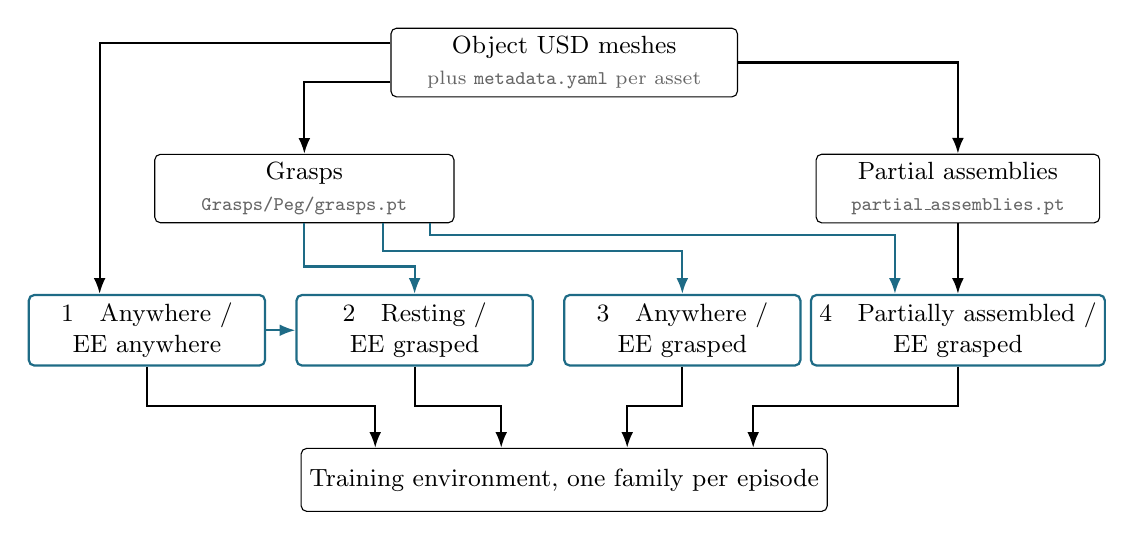
\begin{tikzpicture}[x=1cm, y=1cm]
  \node[blk, minimum width=44mm] (mesh) at (6.9,4.2) {Object USD meshes\\ \subl{plus \code{metadata.yaml} per asset}};
  \node[blk, minimum width=38mm] (grasp) at (3.6,2.6) {Grasps\\ \subl{\code{Grasps/Peg/grasps.pt}}};
  \node[blk, minimum width=36mm] (part) at (11.9,2.6) {Partial assemblies\\ \subl{\code{partial\_assemblies.pt}}};
  \node[blk, key, minimum width=30mm] (f1) at (1.6,0.8) {1\quad Anywhere /\\ EE anywhere};
  \node[blk, key, minimum width=30mm] (f2) at (5.0,0.8) {2\quad Resting /\\ EE grasped};
  \node[blk, key, minimum width=30mm] (f3) at (8.4,0.8) {3\quad Anywhere /\\ EE grasped};
  \node[blk, key, minimum width=30mm] (f4) at (11.9,0.8) {4\quad Partially assembled /\\ EE grasped};
  \node[blk, minimum width=60mm] (train) at (6.9,-1.1) {Training environment, one family per episode};
  % meshes feed grasps, partial assemblies and family 1
  \draw[arr] ([yshift=-2.5mm]mesh.west) -| (grasp.north);
  \draw[arr] (mesh.east) -| (part.north);
  \draw[arr] ([yshift=2.5mm]mesh.west) -| ([xshift=-6mm]f1.north);
  % grasps feed every grasped family
  \draw[karr] (grasp.south) -- ++(0,-0.55) -| (f2.north);
  \draw[karr] ([xshift=10mm]grasp.south) -- ++(0,-0.35) -| (f3.north);
  \draw[karr] ([xshift=16mm]grasp.south) -- ++(0,-0.15) -| ([xshift=-8mm]f4.north);
  % family 1 feeds family 2; partial assemblies feed family 4
  \draw[karr] (f1.east) -- (f2.west);
  \draw[arr] (part.south) -- (f4.north);
  % all four feed training
  \draw[arr] (f1.south) -- ++(0,-0.5) -| ([xshift=-24mm]train.north);
  \draw[arr] (f2.south) -- ++(0,-0.5) -| ([xshift=-8mm]train.north);
  \draw[arr] (f3.south) -- ++(0,-0.5) -| ([xshift=8mm]train.north);
  \draw[arr] (f4.south) -- ++(0,-0.5) -| ([xshift=24mm]train.north);
\end{tikzpicture}
\caption{Dependency graph of the three datasets and the four reset families. Grasps (blue arrows) feed every grasped family. Family~2 additionally draws its object poses from family~1, so family~1 must be recorded first. The pipeline script runs partial assemblies, then grasps, then the four families in numerical order.}
\label{fig:deps}
\end{figure}

\subsection{Partial Assemblies}
\label{sec:partial}

The partial-assembly dataset answers the question ``what does a half-finished insertion look like?'' The procedure places the insertive object exactly at its assembled pose, which the asset metadata provides as an offset relative to the receptive object. It then applies a tiny random force and torque to the object on every physics step, so that the object jiggles out of the hole along whatever directions the geometry allows. At each physics step the pose of the insertive object expressed in the frame of the receptive object is logged. A pose is kept when the objects are collision-free at that instant and when it differs from every pose already kept by more than a position and an orientation threshold. The result is a set of relative poses $(\bm p^{\mathrm{rec}}_{\mathrm{ins}},\bm q^{\mathrm{rec}}_{\mathrm{ins}})$ that span the insertion path. The file does not store a robot state. It stores only where the object may sit in the hole.

\paragraph{Where the assembled pose comes from.}
The sampler does not know what a finished insertion looks like. That knowledge is authored by hand, once per asset, in a small \code{metadata.yaml} file next to each USD. Each object declares an \code{assembled\_offset}, a frame fixed to that object, and the pair is assembled when the two frames coincide. Writing $T_{\mathrm{ins}}$ and $T_{\mathrm{rec}}$ for the two offsets, the insertive object's assembled pose in the world is
\begin{equation}
  \Tf{\w}{\mathrm{ins}} = \Tf{\w}{\mathrm{rec}}\; T_{\mathrm{rec}}\; T_{\mathrm{ins}}^{-1}.
  \label{eq:assembled}
\end{equation}
For the peg the offset is the identity, and for the hole it is a translation of $14.8$\,mm along $z$, which is where the peg's origin sits when it is fully home. The hole's metadata also carries the \code{success\_thresholds}, $2.5$\,mm and $0.025$\,rad, that define a completed insertion, and both files carry a \code{bottom\_offset} that the spawner uses to rest objects on the table. None of these numbers is computed from the meshes.

Suppose, then, that you want to insert a gear between two fixed gears. You would provide the insertive gear as one USD and the fixture with both fixed gears as a single receptive USD, then write the two metadata files so that the assembled offsets coincide exactly at the meshed pose, measured in a USD editor or from the CAD. Only after that can the sampler do its part, which is to perturb the object out of that pose with tiny forces and record every collision-free pose it passes through until its bounding box no longer overlaps the receptive object. The sampler also assumes one assembled pose per pair: a gear has as many valid meshing angles as it has teeth, and only the one you author, plus whatever the perturbation reaches from it, will appear in the dataset. Note too that this environment sets friction to zero on both objects, so forces of $5$\,mN and $5$\,mN\,m suffice to move the part.

\subsection{Grasps}
\label{sec:grasps}

The grasp dataset answers ``how can this gripper hold this object?'' It is recorded with a gripper alone, anchored to the world, and the object floating in front of it. Candidate grasps are generated geometrically by antipodal sampling on the object mesh~\cite{nguyen1988constructing}, in the three steps sketched in Figure~\ref{fig:threesteps}.
\begin{enumerate}[leftmargin=*, itemsep=2pt]
  \item Sample points on the mesh surface, together with their outward normals. A share of the samples is taken from the highest points with upward-facing normals; the rest are uniform over the surface. For the Dex1 gripper this share is one half, so that a peg lying on its side also receives grasps across its diameter.
  \item From each sample, cast a ray into the object along the negative normal. The farthest hit that lies within the gripper's maximum aperture becomes the opposing contact. The segment between the two contacts is the \emph{grasp axis}, and its midpoint is the \emph{grasp centre}.
  \item Align the gripper's alignment axis, which for both grippers here is its approach direction, with the grasp axis, rotate about the approach direction through sixteen equally spaced angles, and for each angle retreat the gripper along its approach direction through thirty-two standoff distances between the finger offset and the finger offset plus the mesh diagonal.
\end{enumerate}

\begin{figure}[tp]
\centering
\resizebox{\linewidth}{!}{%
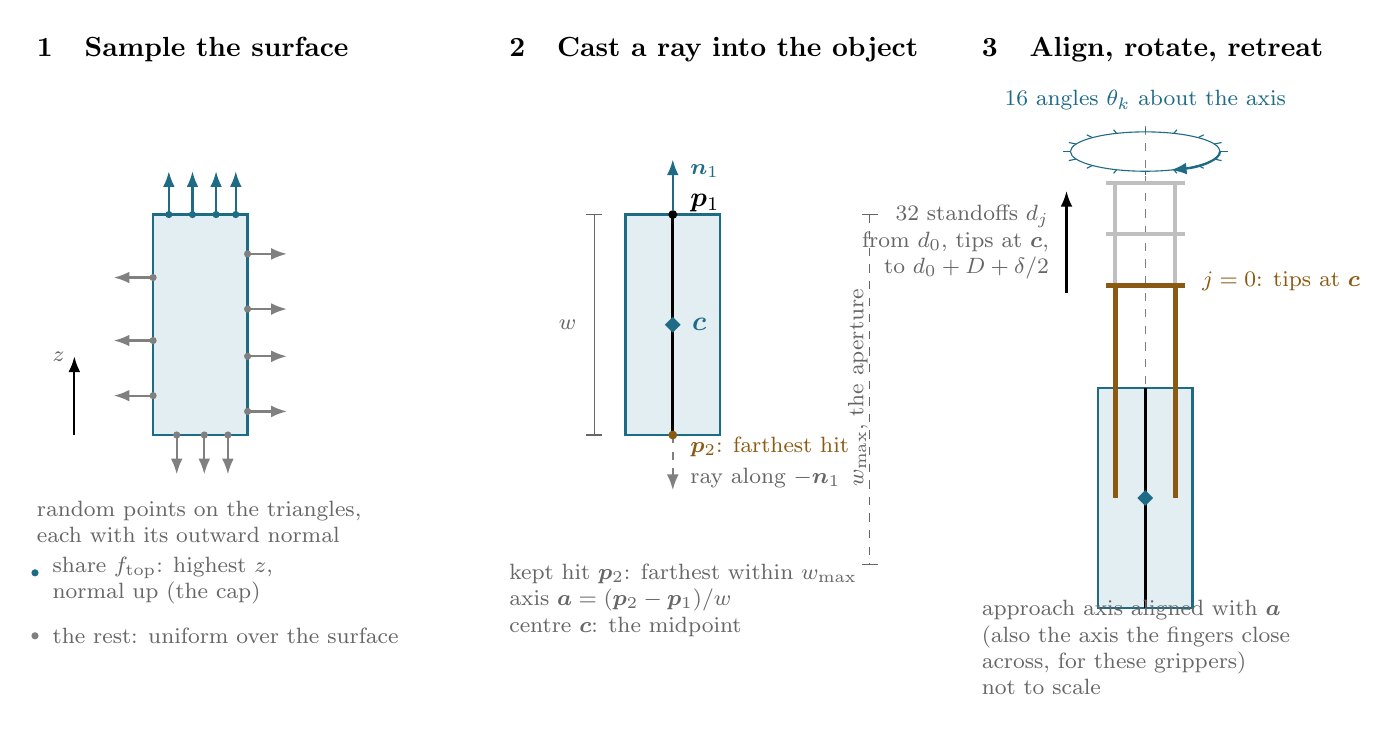
\begin{tikzpicture}[x=1cm, y=1cm, every node/.style={font=\normalsize}, sub/.style={font=\footnotesize\color{black!60}}]
  % ---------------- panel 1: sample
  \node[font=\normalsize\bfseries, anchor=west] at (0,5.9) {1\quad Sample the surface};
  \fill[accentsoft] (1.6,1.0) rectangle (2.8,3.8); \draw[accent, thick] (1.6,1.0) rectangle (2.8,3.8);
  \draw[arr] (0.6,1.0) -- (0.6,2.0); \node[sub, left] at (0.6,2.0) {$z$};
  \foreach \x in {1.8,2.1,2.4,2.65} {\fill[accent] (\x,3.8) circle (1.3pt); \draw[karr] (\x,3.82) -- (\x,4.35);}
  \foreach \y in {1.5,2.2,3.0} {\fill[black!50] (1.6,\y) circle (1.3pt); \draw[arr, black!50] (1.58,\y) -- (1.1,\y);}
  \foreach \y in {1.3,2.0,2.6,3.3} {\fill[black!50] (2.8,\y) circle (1.3pt); \draw[arr, black!50] (2.82,\y) -- (3.3,\y);}
  \foreach \x in {1.9,2.25,2.55} {\fill[black!50] (\x,1.0) circle (1.3pt); \draw[arr, black!50] (\x,0.98) -- (\x,0.5);}
  \node[sub, anchor=west, align=left] at (0,-0.1) {random points on the triangles,\\ each with its outward normal};
  \fill[accent] (0.1,-0.75) circle (1.3pt); \node[sub, anchor=west, align=left] at (0.2,-0.85) {share $f_{\mathrm{top}}$: highest $z$,\\ normal up (the cap)};
  \fill[black!50] (0.1,-1.55) circle (1.3pt); \node[sub, anchor=west, align=left] at (0.2,-1.55) {the rest: uniform over the surface};
  % ---------------- panel 2: ray
  \begin{scope}[shift={(6.0,0)}]
  \node[font=\normalsize\bfseries, anchor=west] at (0,5.9) {2\quad Cast a ray into the object};
  \fill[accentsoft] (1.6,1.0) rectangle (2.8,3.8); \draw[accent, thick] (1.6,1.0) rectangle (2.8,3.8);
  \fill (2.2,3.8) circle (1.6pt); \node[anchor=west] at (2.3,3.95) {$\bm p_1$};
  \draw[karr] (2.2,3.85) -- (2.2,4.5); \node[sub, accent, anchor=west] at (2.3,4.35) {$\bm n_1$};
  \draw[very thick] (2.2,3.75) -- (2.2,1.05);
  \draw[arr, dashed, black!50] (2.2,1.0) -- (2.2,0.3); \node[sub, anchor=west] at (2.3,0.45) {ray along $-\bm n_1$};
  \fill[warn] (2.2,1.0) circle (1.6pt); \node[sub, warn, anchor=west] at (2.3,0.85) {$\bm p_2$: farthest hit};
  \fill[accent] (2.2,2.4) ++(0,0.1) -- ++(0.1,-0.1) -- ++(-0.1,-0.1) -- ++(-0.1,0.1) -- cycle; \node[accent, anchor=west] at (2.32,2.4) {$\bm c$};
  \draw[black!60] (1.2,1.0) -- (1.2,3.8); \draw[black!60] (1.1,1.0) -- (1.3,1.0); \draw[black!60] (1.1,3.8) -- (1.3,3.8); \node[sub, anchor=east] at (1.1,2.4) {$w$};
  \draw[black!60, dashed] (4.7,3.8) -- (4.7,-0.65); \draw[black!60] (4.6,3.8) -- (4.8,3.8); \draw[black!60] (4.6,-0.65) -- (4.8,-0.65);
  \node[sub, rotate=90, anchor=south] at (4.8,1.6) {$w_{\max}$, the aperture};
  \node[sub, anchor=west, align=left] at (0,-1.1) {kept hit $\bm p_2$: farthest within $w_{\max}$\\ axis $\bm a=(\bm p_2-\bm p_1)/w$\\ centre $\bm c$: the midpoint};
  \end{scope}
  % ---------------- panel 3: align, rotate, retreat
  \begin{scope}[shift={(12.0,0)}]
  \node[font=\normalsize\bfseries, anchor=west] at (0,5.9) {3\quad Align, rotate, retreat};
  \fill[accentsoft] (1.6,-1.2) rectangle (2.8,1.6); \draw[accent, thick] (1.6,-1.2) rectangle (2.8,1.6);
  \draw[very thick] (2.2,1.6) -- (2.2,-1.2);
  \draw[black!50, dashed] (2.2,1.65) -- (2.2,5.0);
  \fill[accent] (2.2,0.2) ++(0,0.1) -- ++(0.1,-0.1) -- ++(-0.1,-0.1) -- ++(-0.1,0.1) -- cycle;
  % ghost grippers
  \foreach \dy in {1.3,0.65} {\draw[black!25, line width=1.4pt] (1.7,2.9+\dy) -- (2.7,2.9+\dy) (1.82,2.9+\dy) -- (1.82,0.2+\dy) (2.58,2.9+\dy) -- (2.58,0.2+\dy);}
  % gripper at j = 0
  \draw[warn, line width=1.8pt] (1.7,2.9) -- (2.7,2.9) (1.82,2.9) -- (1.82,0.2) (2.58,2.9) -- (2.58,0.2);
  \node[sub, warn, anchor=west] at (2.8,2.95) {$j=0$: tips at $\bm c$};
  % rotation about the axis
  \draw[accent] (2.2,4.6) ellipse (0.95 and 0.25);
  \foreach \a in {0,22.5,...,337.5} {\draw[accent] ($(2.2,4.6)+({0.95*cos(\a)},{0.25*sin(\a)})$) -- ($(2.2,4.6)+({1.05*cos(\a)},{0.3*sin(\a)})$);}
  \draw[karr] (3.15,4.6) arc[start angle=0, end angle=-70, x radius=0.95, y radius=0.25];
  \node[sub, accent, anchor=south] at (2.2,5.0) {16 angles $\theta_k$ about the axis};
  % retreat arrow
  \draw[arr] (1.2,2.8) -- (1.2,4.1);
  \node[sub, anchor=east, align=right] at (1.1,3.45) {32 standoffs $d_j$\\ from $d_0$, tips at $\bm c$,\\ to $d_0+D+\delta/2$};
  \node[sub, anchor=west, align=left] at (0,-1.7) {approach axis aligned with $\bm a$\\ (also the axis the fingers close\\ across, for these grippers)\\ not to scale};
  \end{scope}
\end{tikzpicture}}
\caption{The three construction steps on a block, side view. Left: surface samples with their outward normals, the top-biased share in blue and the uniform share in grey. Middle: one sample casts a ray along its inward normal; the farthest hit within the aperture is the opposing contact, and the segment between the two is the grasp axis with the centre at its midpoint. Right: the gripper's approach axis is aligned with the grasp axis, rolled through sixteen angles about it, and retreated along it through thirty-two standoffs, the nearest of which puts the fingertips at the centre.}
\label{fig:threesteps}
\end{figure}

\paragraph{Choosing surface points.}
The budget is a number of candidates, $N_{\mathrm{cand}}=10^6$, which is divided among the orientations and standoffs to give the number of surface samples,
\begin{equation}
  N_{\mathrm{surf}} = \Big\lfloor \frac{N_{\mathrm{cand}}}{n_\theta\, n_d} \Big\rfloor = \Big\lfloor \frac{10^6}{16\times 32} \Big\rfloor = 1953 .
\end{equation}
Ten times that many points are drawn uniformly on the mesh, each with its face normal $\bm n_i$, and every point receives a top-bias score in the object's own frame,
\begin{equation}
  s_i = \frac{z_i - z_{\min}}{z_{\max}-z_{\min}} + \max(n_{i,z},\,0),
  \label{eq:topbias}
\end{equation}
which is largest for high points whose normals face up. A fraction $f_{\mathrm{top}}$ of the $N_{\mathrm{surf}}$ samples is taken from the top of this ranking and the remainder uniformly from the rest. The Robotiq configuration uses $f_{\mathrm{top}}=1$; the Dex1 configuration uses $f_{\mathrm{top}}=0.5$, for the reason shown in Figure~\ref{fig:sidegrasp}.

\paragraph{The antipodal pair.}
From a sample $\bm p_1$ with outward normal $\bm n_1$, a ray is cast into the object, $\bm r(t)=\bm p_1 - t\,\bm n_1$ for $t>0$. Among its intersections with the mesh, the opposing contact is the farthest one that the gripper can still span,
\begin{equation}
  \bm p_2 = \arg\max_{\bm p\in\text{hits}} \lVert \bm p-\bm p_1\rVert
  \quad\text{subject to}\quad \lVert \bm p-\bm p_1\rVert \le w_{\max},
\end{equation}
where $w_{\max}$ is the gripper's maximum aperture from its metadata, $9.0$\,cm for the Robotiq and $9.5$\,cm for the Dex1. A sample with no admissible hit is discarded. The pair defines the grasp width, axis and centre,
\begin{equation}
  w = \lVert \bm p_2-\bm p_1\rVert, \qquad \bm a = \frac{\bm p_2-\bm p_1}{w}, \qquad \bm c = \bm p_1 + \tfrac{w}{2}\,\bm a .
  \label{eq:pair}
\end{equation}
Choosing the farthest hit rather than the nearest makes the segment span the whole object along that line, so the centre lies in the middle of the body rather than inside a thin wall.

\paragraph{From a pair to a family of gripper poses.}
A gripper's metadata names three unit vectors in its own base frame: the approach direction $\bm g_{\mathrm{app}}$, the axis $\bm g_{\mathrm{al}}$ to be aligned with the grasp axis, and the axis $\bm o$ about which orientations are sampled. For both grippers in this repository all three are the base frame's $x$ axis, which points from the palm to the fingertips. The candidate transforms are
\begin{align}
  T_{k,j} &= \operatorname{Trans}(\bm c)\; R_{\mathrm{al}}\; \operatorname{Rot}(\bm o,\theta_k)\; \operatorname{Trans}(-d_j\,\bm g_{\mathrm{app}}), \label{eq:candidate}\\
  \theta_k &= -\pi + \frac{2\pi k}{n_\theta-1},\quad k=0,\dots,15; \qquad
  d_j = d_0 + \frac{j}{n_d-1}\Big(D+\tfrac{\delta}{2}\Big),\quad j=0,\dots,31, \nonumber
\end{align}
where $R_{\mathrm{al}}$ is the rotation that takes $\bm g_{\mathrm{al}}$ onto $\bm a$, $d_0$ is the \emph{finger offset}, the distance from the gripper base to the fingertips ($13.45$\,cm for the Robotiq, $12$\,cm for the Dex1), $D$ is the diagonal of the object's bounding box, and $\delta$ is the \emph{finger clearance} ($6.0$\,cm and $6.6$\,cm). Because the approach direction and the alignment axis coincide, the construction has a simple geometric reading (Figure~\ref{fig:antipodal}). The gripper approaches along the line through $\bm p_1$ and $\bm p_2$, with $\bm p_1$ nearest the palm, and its fingers close across that line. The sixteen angles $\theta_k$ spin the closing direction around the line, and the thirty-two standoffs slide the fingertips along it, from the segment's centre at $j=0$ outward past $\bm p_1$ at large $j$.

\begin{figure}[t]
\centering
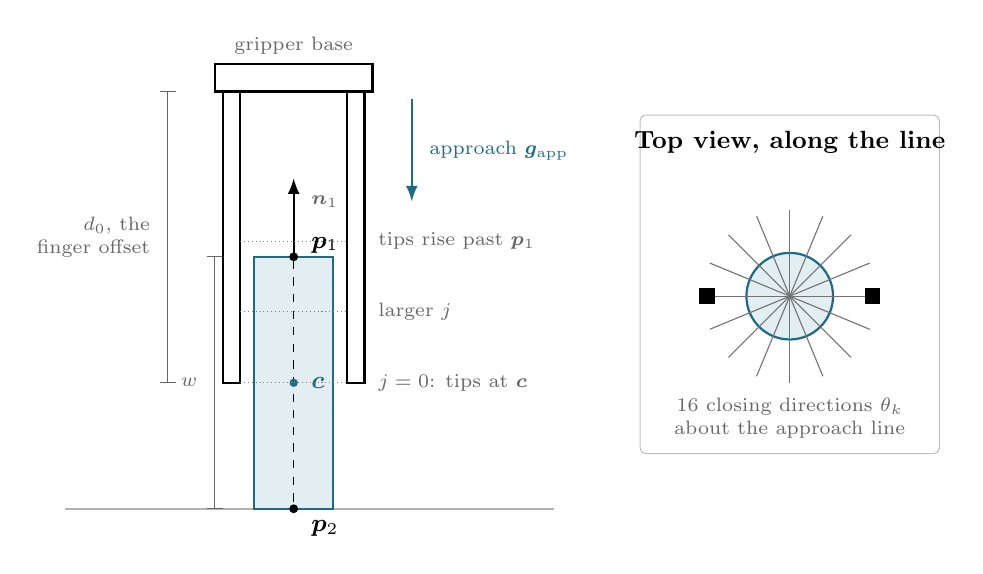
\begin{tikzpicture}[x=1cm, y=1cm]
  % side view
  \draw[black!30, thick] (0.2,0) -- (6.4,0);
  \fill[accentsoft] (2.6,0) rectangle (3.6,3.2); \draw[accent, thick] (2.6,0) rectangle (3.6,3.2);
  \fill (3.1,3.2) circle (1.6pt); \node[font=\small, anchor=west] at (3.2,3.35) {$\bm p_1$};
  \draw[arr] (3.1,3.2) -- (3.1,4.2); \node[sub, anchor=west] at (3.2,3.9) {$\bm n_1$};
  \draw[dashed] (3.1,3.15) -- (3.1,0.05);
  \fill (3.1,0) circle (1.6pt); \node[font=\small, anchor=west] at (3.2,-0.25) {$\bm p_2$};
  \fill[accent] (3.1,1.6) circle (1.5pt); \node[font=\small, accent, anchor=west] at (3.2,1.6) {$\bm c$};
  \draw[black!60] (2.1,0) -- (2.1,3.2); \draw[black!60] (2.0,0) -- (2.2,0); \draw[black!60] (2.0,3.2) -- (2.2,3.2);
  \node[sub, anchor=east] at (2.0,1.6) {$w$};
  % gripper
  \draw[thick, fill=white] (2.1,5.3) rectangle (4.1,5.65); \node[sub, above] at (3.1,5.65) {gripper base};
  \draw[thick, fill=white] (2.2,1.6) rectangle (2.42,5.3);
  \draw[thick, fill=white] (3.78,1.6) rectangle (4.0,5.3);
  \draw[karr] (4.6,5.2) -- (4.6,3.9); \node[sub, accent, anchor=west] at (4.7,4.55) {approach $\bm g_{\mathrm{app}}$};
  \draw[black!60] (1.5,1.6) -- (1.5,5.3); \draw[black!60] (1.4,1.6) -- (1.6,1.6); \draw[black!60] (1.4,5.3) -- (1.6,5.3);
  \node[sub, anchor=east, align=right] at (1.4,3.45) {$d_0$, the\\ finger offset};
  \draw[black!50, densely dotted] (2.42,1.6) -- (3.78,1.6); \node[sub, anchor=west] at (4.05,1.6) {$j=0$: tips at $\bm c$};
  \draw[black!50, densely dotted] (2.42,2.5) -- (3.78,2.5); \node[sub, anchor=west] at (4.05,2.5) {larger $j$};
  \draw[black!50, densely dotted] (2.42,3.4) -- (3.78,3.4); \node[sub, anchor=west] at (4.05,3.4) {tips rise past $\bm p_1$};
  % inset: top view
  \begin{scope}[shift={(9.4,2.7)}]
    \draw[black!25, rounded corners=2pt] (-1.9,-2.0) rectangle (1.9,2.3);
    \node[font=\small\bfseries] at (0,1.95) {Top view, along the line};
    \fill[accentsoft] (0,0) circle (0.55); \draw[accent, thick] (0,0) circle (0.55);
    \foreach \ang in {0,22.5,...,157.5} { \draw[black!55] (\ang:1.1) -- (\ang+180:1.1); }
    \fill (-1.15,-0.1) rectangle (-0.95,0.1); \fill (0.95,-0.1) rectangle (1.15,0.1);
    \node[sub, align=center] at (0,-1.55) {16 closing directions $\theta_k$\\ about the approach line};
  \end{scope}
\end{tikzpicture}
\caption{The antipodal construction on a standing peg. The sample $\bm p_1$ on the top cap casts a ray along its inward normal to $\bm p_2$ on the bottom. The gripper approaches along that line, its fingers close across it, the standoffs slide the fingertips from the centre upward, and the inset shows the sixteen closing directions sampled about the line.}
\label{fig:antipodal}
\end{figure}

\begin{figure}[t]
\centering
\resizebox{\linewidth}{!}{%
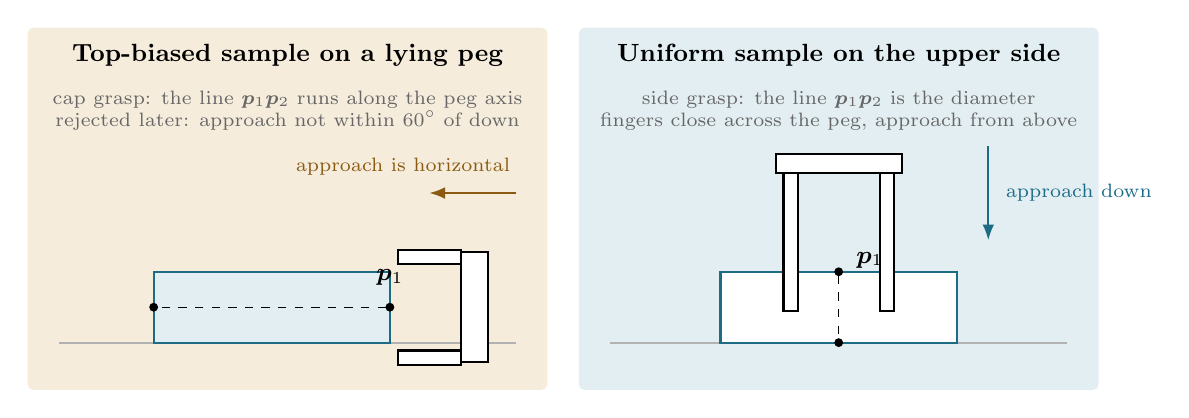
\begin{tikzpicture}[x=1cm, y=1cm]
  % left panel: cap grasp on a lying peg
  \fill[warnsoft, rounded corners=2pt] (0,0) rectangle (6.6,4.6);
  \node[font=\small\bfseries] at (3.3,4.25) {Top-biased sample on a lying peg};
  \node[sub, align=center] at (3.3,3.55) {cap grasp: the line $\bm p_1\bm p_2$ runs along the peg axis\\ rejected later: approach not within $60^\circ$ of down};
  \draw[black!30, thick] (0.4,0.6) -- (6.2,0.6);
  \fill[accentsoft] (1.6,0.6) rectangle (4.6,1.5); \draw[accent, thick] (1.6,0.6) rectangle (4.6,1.5);
  \fill (4.6,1.05) circle (1.6pt); \node[font=\small, above] at (4.6,1.2) {$\bm p_1$};
  \draw[dashed] (4.55,1.05) -- (1.65,1.05); \fill (1.6,1.05) circle (1.6pt);
  \draw[thick, fill=white] (5.5,0.35) rectangle (5.85,1.75);
  \draw[thick, fill=white] (4.7,1.6) rectangle (5.5,1.78); \draw[thick, fill=white] (4.7,0.32) rectangle (5.5,0.5);
  \draw[-{Latex[length=2mm]}, thick, warn] (6.2,2.5) -- (5.1,2.5); \node[sub, warn, anchor=south east] at (6.25,2.6) {approach is horizontal};
  % right panel: side sample
  \fill[accentsoft, rounded corners=2pt] (7.0,0) rectangle (13.6,4.6);
  \node[font=\small\bfseries] at (10.3,4.25) {Uniform sample on the upper side};
  \node[sub, align=center] at (10.3,3.55) {side grasp: the line $\bm p_1\bm p_2$ is the diameter\\ fingers close across the peg, approach from above};
  \draw[black!30, thick] (7.4,0.6) -- (13.2,0.6);
  \fill[white] (8.8,0.6) rectangle (11.8,1.5); \draw[accent, thick] (8.8,0.6) rectangle (11.8,1.5);
  \fill (10.3,1.5) circle (1.6pt); \node[font=\small, anchor=west] at (10.4,1.65) {$\bm p_1$};
  \draw[dashed] (10.3,1.45) -- (10.3,0.65); \fill (10.3,0.6) circle (1.6pt);
  \draw[thick, fill=white] (9.5,2.75) rectangle (11.1,3.0);
  \draw[thick, fill=white] (9.6,1.0) rectangle (9.78,2.75); \draw[thick, fill=white] (10.82,1.0) rectangle (11.0,2.75);
  \draw[karr] (12.2,3.1) -- (12.2,1.9); \node[sub, accent, anchor=west] at (12.3,2.5) {approach down};
\end{tikzpicture}}
\caption{Why the Dex1 sampler takes half of its surface points uniformly. The top-bias score of Eq.~\eqref{eq:topbias}, computed in the object frame, prefers the end caps of the peg. Those grasps approach along the peg axis, which is horizontal for a peg lying on the table, and the reset-state test rejects any hand that does not point within $60^\circ$ of down. A sample on the upper side of the lying peg gives a vertical approach with the fingers across the diameter.}
\label{fig:sidegrasp}
\end{figure}

Every candidate is a rigid transform $\Tf{\obj}{\grip}$ of the gripper in the object frame. At each reset the environment opens the fingers, teleports the anchored gripper to a random candidate around the object, and commands the fingers closed. Gravity is switched on after one second and small disturbance forces are applied. The episode lasts four seconds. A candidate becomes a recorded grasp when, at the end, the object has moved less than a quarter metre from where it started, is still above half the spawn height, is not interpenetrating the gripper, has settled, and the fingers have travelled at least ten percent of the way from open to closed. The last clause rejects an object that merely rests across fully open fingers. The recorder saves the gripper pose in the object frame and the finger joint positions.

\paragraph{Physical validation.}
Geometry proposes and physics disposes. Each candidate is tried in simulation, and the grasp recorder keeps it only if, at the end of the four-second episode, every one of the following holds: the object's centre has moved less than $25$\,cm from where it started, it is still above $25$\,cm (half the spawn height), neither body is moving, the gripper's point cloud is at least half a millimetre clear of the object, and the fingers have travelled at least a tenth of their range,
\begin{equation}
  f_{\mathrm{close}} = \frac{\theta-\theta_{\mathrm{open}}}{\theta_{\mathrm{closed}}-\theta_{\mathrm{open}}} > 0.1 .
\end{equation}
Only a small fraction of the geometric candidates survive. On the peg with the Dex1, one run of the recorder with $256$ environments collected $97$ grasps, $80$ of them on the caps and $17$ across the body, and $8$ of those $17$ were later dropped at load time because the fingers had stayed open.

\paragraph{No learned grasp model is involved.}
There is no GraspNet, Contact-GraspNet, AnyGrasp or Dex-Net anywhere in this pipeline. Candidates come from the antipodal construction above and are filtered by simulation alone. This is a deliberate fit for the task: the objects are few, their meshes are exact, and a full physics engine is available to try every candidate, so a learned prior would add a dependency without adding information. The dataset format is nothing more than a list of gripper poses in the object frame with finger positions, so a learned planner could be dropped in as an alternative candidate source without touching the reset-state generator.

\subsection{A Worked Run on the Peg, Stage by Stage}
\label{sec:worked}

The equations above are easier to believe once the stages have been seen. The figures in this subsection come from re-running the sampler's own code on \path{Props/Custom/Peg/peg.usd} with the Dex1 metadata, and from the grasp file the recorder wrote for that peg. The peg is a plain block of $3\times3\times6$\,cm with $z$ along its length, and everything is drawn in the peg's own frame because that is the frame the grasp file uses. Figure~\ref{fig:graspblocks} shows the whole procedure as blocks with the counts from this run.

\begin{figure}[tp]
\centering
\resizebox{\linewidth}{!}{%
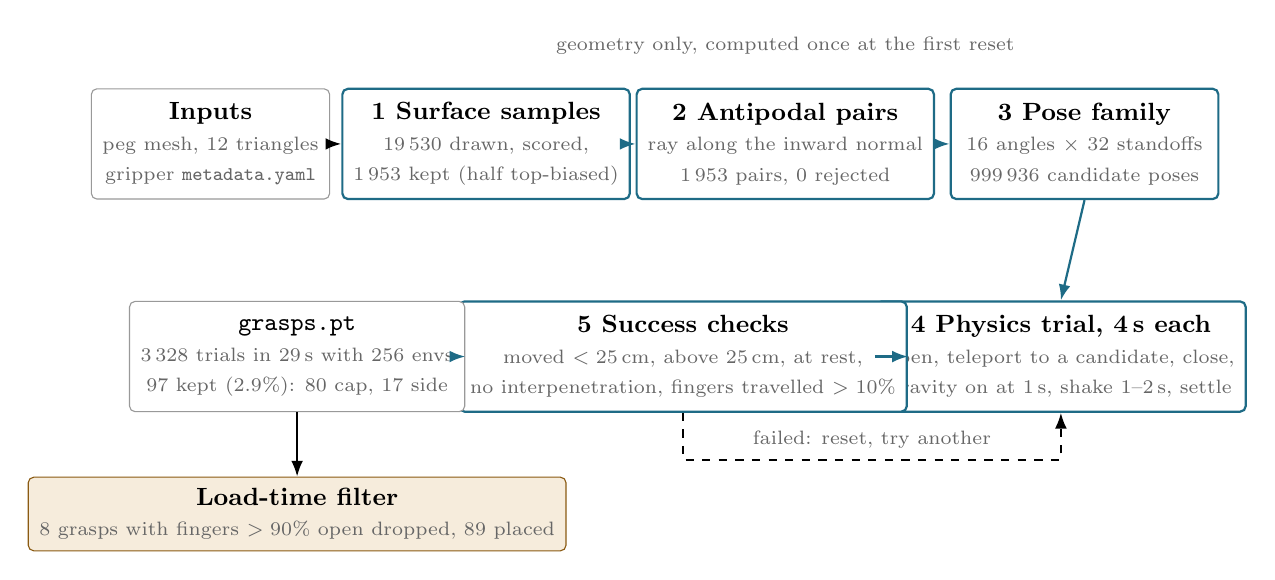
\begin{tikzpicture}[x=1cm, y=1cm,
  st/.style={draw=accent, thick, fill=white, rounded corners=2pt, align=center, inner sep=4pt, font=\small, minimum height=14mm},
  io/.style={draw=black!40, fill=white, rounded corners=2pt, align=center, inner sep=4pt, font=\small, minimum height=14mm},
  bad/.style={draw=warn, fill=warnsoft, rounded corners=2pt, align=center, inner sep=4pt, font=\small}]
  \node[io, minimum width=28mm] (in) at (1.5,3) {\textbf{Inputs}\\ \subl{peg mesh, 12 triangles}\\ \subl{gripper \code{metadata.yaml}}};
  \node[st, minimum width=34mm] (s1) at (5.0,3) {\textbf{1 Surface samples}\\ \subl{19\,530 drawn, scored,}\\ \subl{1\,953 kept (half top-biased)}};
  \node[st, minimum width=34mm] (s2) at (8.8,3) {\textbf{2 Antipodal pairs}\\ \subl{ray along the inward normal}\\ \subl{1\,953 pairs, 0 rejected}};
  \node[st, minimum width=34mm] (s3) at (12.6,3) {\textbf{3 Pose family}\\ \subl{16 angles $\times$ 32 standoffs}\\ \subl{999\,936 candidate poses}};
  \node[st, minimum width=40mm] (s4) at (12.3,0.3) {\textbf{4 Physics trial, 4\,s each}\\ \subl{open, teleport to a candidate, close,}\\ \subl{gravity on at 1\,s, shake 1--2\,s, settle}};
  \node[st, minimum width=40mm] (s5) at (7.5,0.3) {\textbf{5 Success checks}\\ \subl{moved $<25$\,cm, above $25$\,cm, at rest,}\\ \subl{no interpenetration, fingers travelled $>10\%$}};
  \node[io, minimum width=40mm] (out) at (2.6,0.3) {\textbf{\code{grasps.pt}}\\ \subl{3\,328 trials in 29\,s with 256 envs}\\ \subl{97 kept (2.9\%): 80 cap, 17 side}};
  \node[bad, minimum width=60mm] (filt) at (2.6,-1.7) {\textbf{Load-time filter}\\ \subl{8 grasps with fingers $>90\%$ open dropped, 89 placed}};
  \draw[arr] (in) -- (s1); \draw[karr] (s1) -- (s2); \draw[karr] (s2) -- (s3);
  \draw[karr] (s3.south) -- (s4.north);
  \draw[karr] (s4) -- (s5); \draw[karr] (s5) -- (out);
  \draw[arr] (out) -- (filt);
  \draw[darr] (s5.south) -- ++(0,-0.6) -| (s4.south);
  \node[sub] at (9.9,-0.75) {failed: reset, try another};
  \node[sub] at (8.8,4.25) {geometry only, computed once at the first reset};
\end{tikzpicture}}
\caption{Grasp generation as blocks, with the counts from the peg run. Steps 1 to 3 are pure geometry and run once; steps 4 and 5 run in the simulator, one candidate per environment per episode, until the requested number of grasps has been recorded.}
\label{fig:graspblocks}
\end{figure}

\paragraph{Sampling the surface.}
``Sample points on the mesh surface'' means picking random points on the triangles, weighted by triangle area, each carrying the outward normal of its triangle. The sampler draws ten times the $1\,953$ it will keep. Figure~\ref{fig:wsamples} shows the samples and their normals; on a box the normals fall into six families. Figure~\ref{fig:wtopbias} shows the top-bias score of Eq.~\eqref{eq:topbias} and the two selections, Dex1 with half of the samples from the top of the ranking and Robotiq with all of them.

\begin{figure}[tp]
\centering
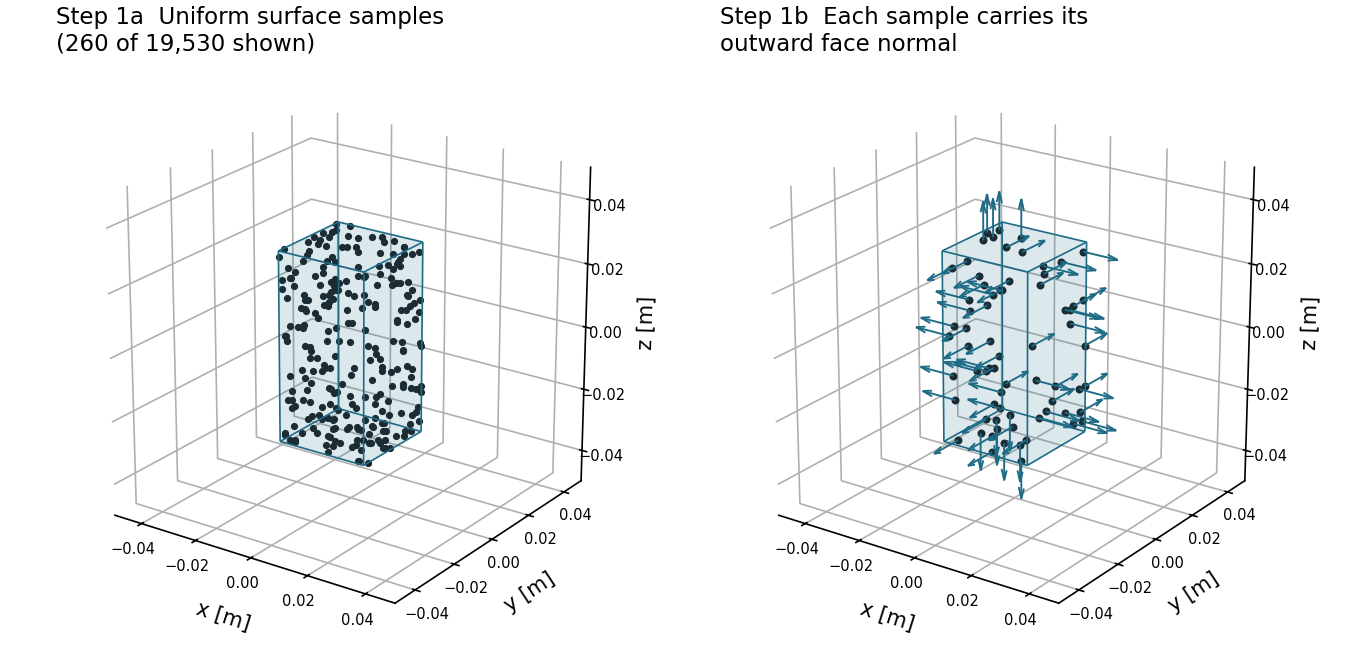
\includegraphics[width=\linewidth]{figures/grasp_f1_samples.png}
\caption{Left: 260 of the 19\,530 uniform surface samples. Right: 70 of them with their outward normals.}
\label{fig:wsamples}
\end{figure}

\begin{figure}[tp]
\centering
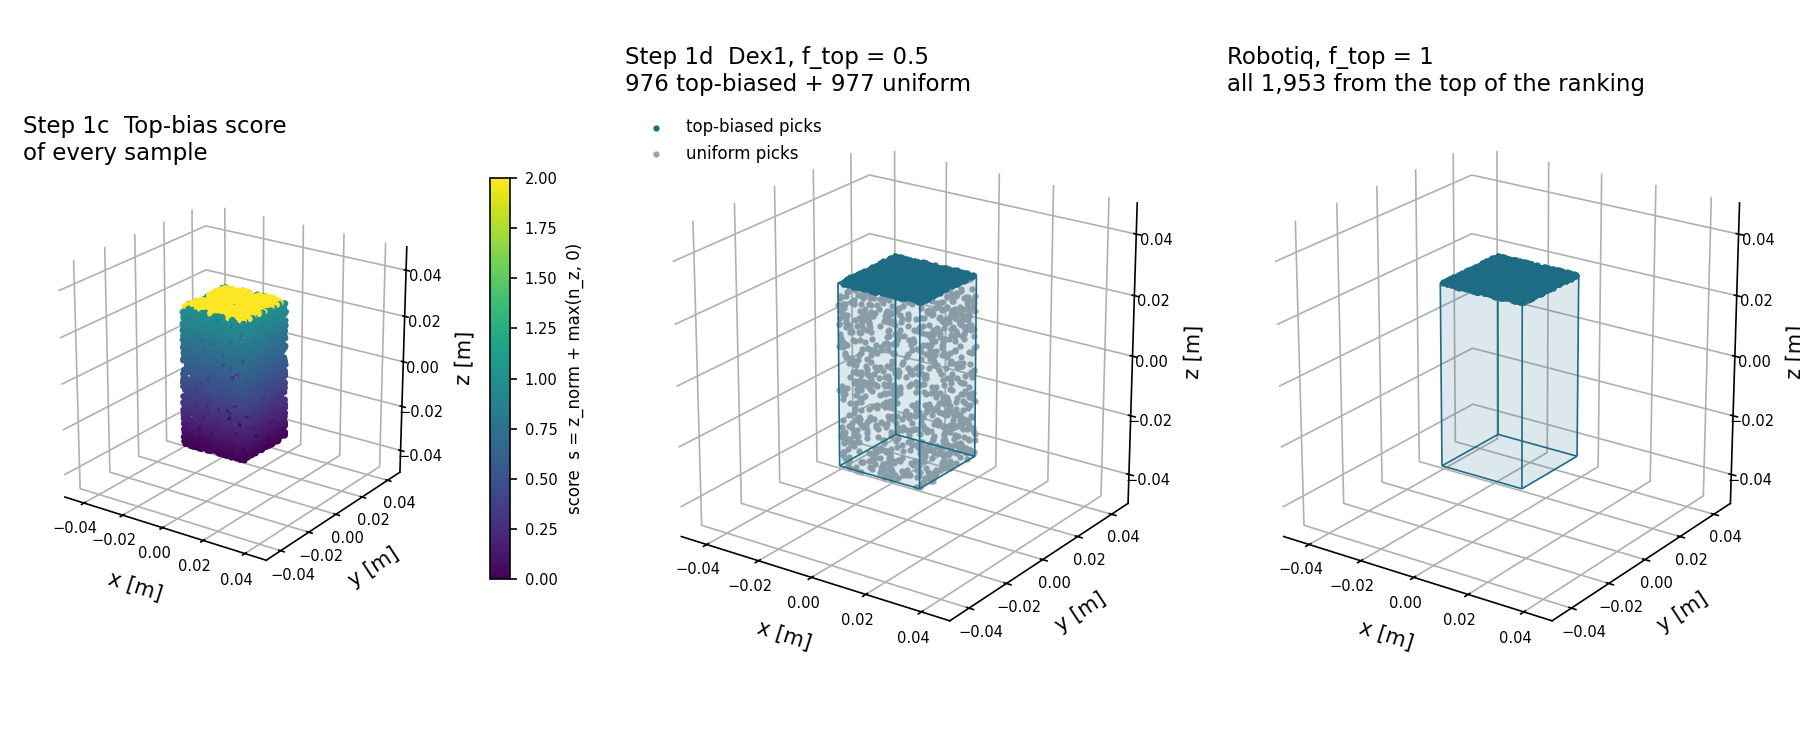
\includegraphics[width=\linewidth]{figures/grasp_f2_topbias.png}
\caption{Left: the top-bias score, from 0 at the bottom to 2 on the top face. Middle: the Dex1 selection, 976 top-biased samples on the cap (blue) and 977 uniform samples (grey). Right: the Robotiq selection, the cap alone. This single difference is why the Dex1 file contains side grasps and the Robotiq file does not.}
\label{fig:wtopbias}
\end{figure}

\paragraph{Casting the ray.}
From a cap sample the ray runs the full $6$\,cm down the peg's axis; from a side sample it crosses the $3$\,cm width. Both are far inside the $9.48$\,cm aperture, so on this peg no sample is rejected (Figure~\ref{fig:wrays}). A longer object would lose its end-cap samples at this step.

\begin{figure}[tp]
\centering
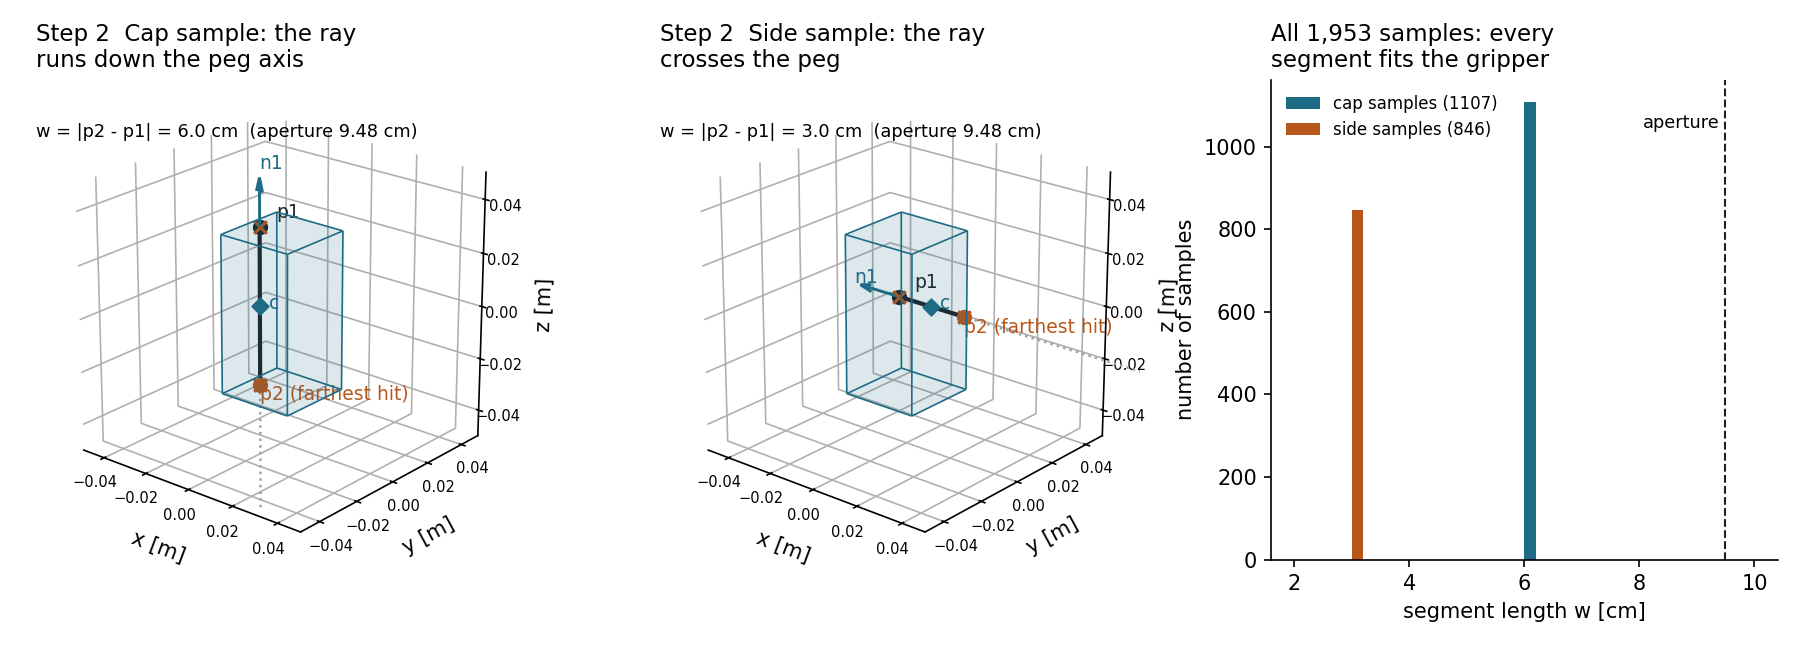
\includegraphics[width=\linewidth]{figures/grasp_f3_rays.png}
\caption{Left and middle: one cap and one side sample, with the ray, the hits, the farthest admissible hit $\bm p_2$ and the centre $\bm c$. Right: the segment lengths of all 1\,953 samples against the aperture.}
\label{fig:wrays}
\end{figure}

\paragraph{Orientations and standoffs.}
Figure~\ref{fig:wstandoff} takes the cap pair of Figure~\ref{fig:wrays} and shows the two sweeps of Eq.~\eqref{eq:candidate}: the 32 gripper-base positions along the approach line, from fingertips at the centre to fingertips $10.6$\,cm above the top of the peg, and the 16 finger-closing directions seen down the line, only two of which can pinch a square peg. Figure~\ref{fig:wcloud} shows all 999\,936 candidates at once. They form six blocks around the peg, above and below it from the cap samples and on four sides from the side samples. Nothing has been tested yet, and the geometry has no notion of up.

\begin{figure}[tp]
\centering
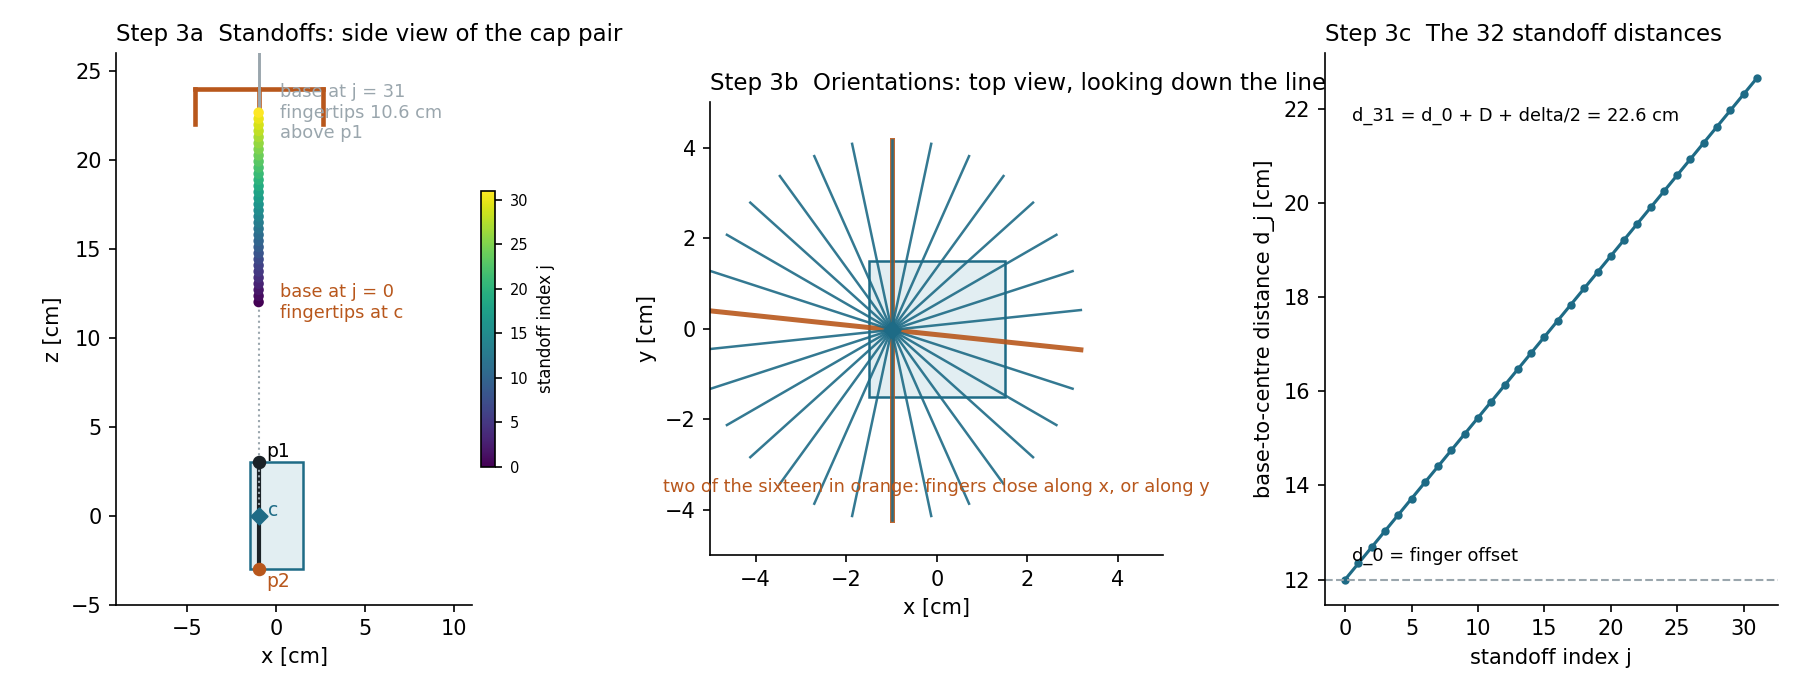
\includegraphics[width=\linewidth]{figures/grasp_f4_orient_standoff.png}
\caption{Left: the standoff sweep for the cap pair, with the gripper drawn at the nearest standoff, fingertips at $\bm c$, and at the farthest. Middle: the 16 closing directions through $\bm c$. Right: the standoff schedule $d_j$.}
\label{fig:wstandoff}
\end{figure}

\begin{figure}[tp]
\centering
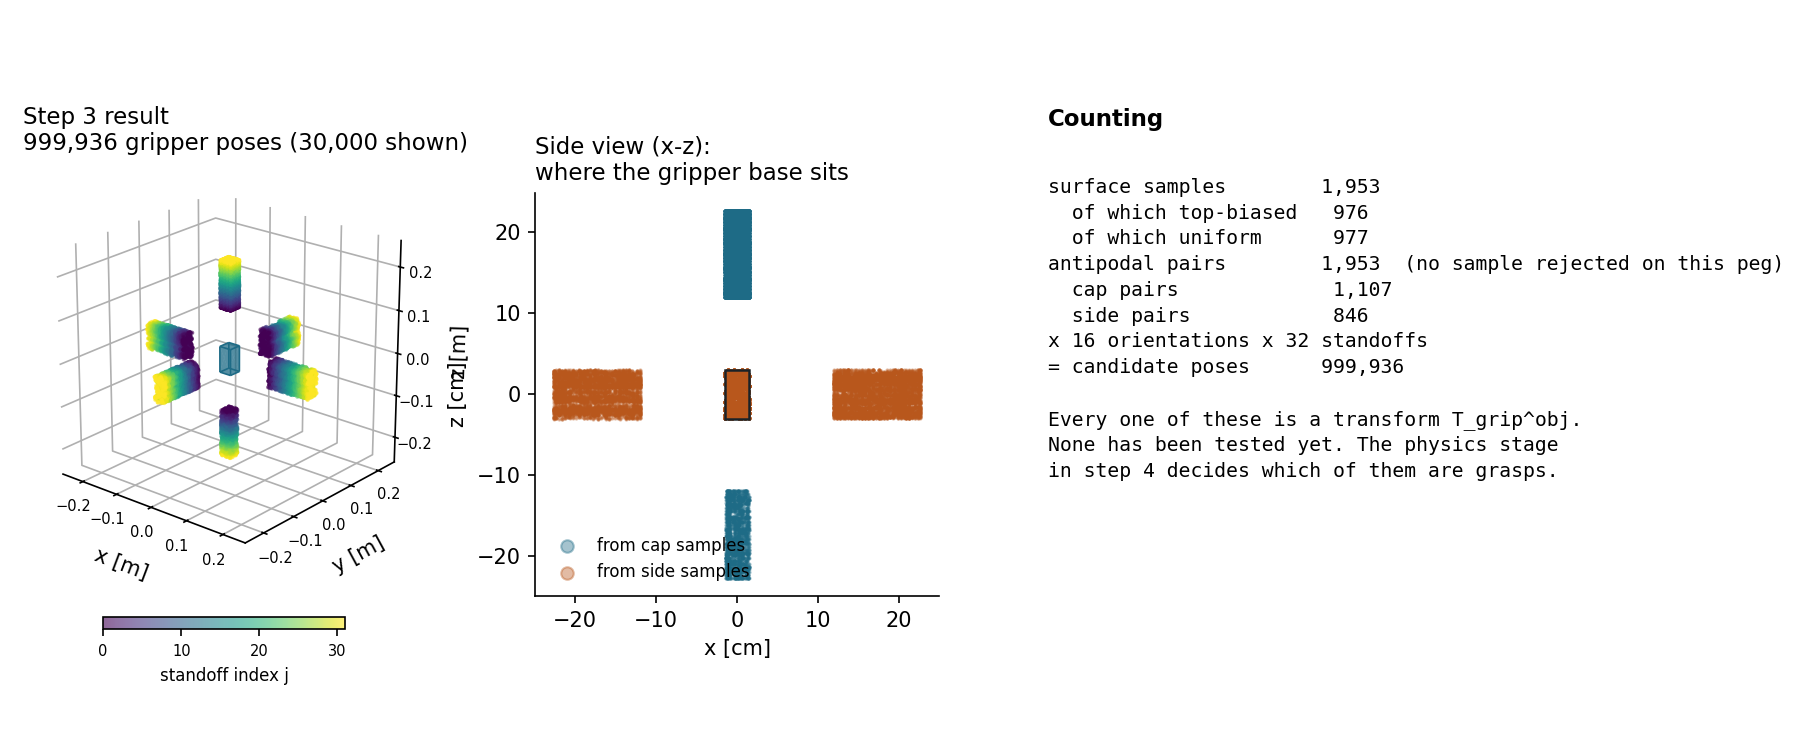
\includegraphics[width=\linewidth]{figures/grasp_f5_candidates.png}
\caption{Every candidate gripper-base position, coloured by standoff index on the left and by sample type in the side view.}
\label{fig:wcloud}
\end{figure}

\paragraph{The trial and the survivors.}
Each candidate is tested in a four-second episode (Figure~\ref{fig:trial}): the fingers open, the anchored gripper is teleported to the candidate with gravity off, the close command is held, gravity comes on at one second, a random force and torque of $0.01$\,N and $0.01$\,N\,m shake the peg between one and two seconds, and the peg then settles or falls away. The recorder tried $3\,328$ candidates in $29$ seconds and kept $97$ (Figure~\ref{fig:wsurvivors}). The survivors cluster at the standoffs where the fingertips straddle the peg. Five of the cap grasps approach from below; they are valid in free space but useless on a table, and the reset-state test later rejects them with its ``approach within $60^\circ$ of down'' clause. Eight grasps ended with the fingers more than $90\%$ open, meaning they closed on nothing, and those are dropped when the file is loaded.

\begin{figure}[tp]
\centering
\resizebox{\linewidth}{!}{%
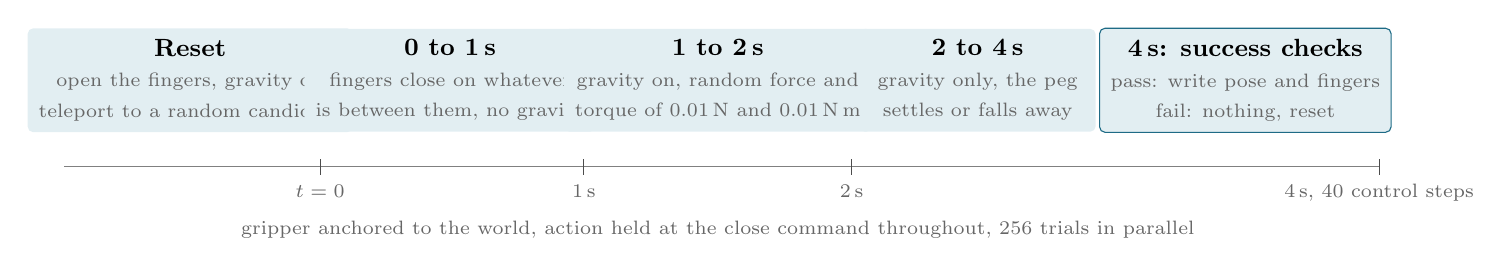
\begin{tikzpicture}[x=1cm, y=1cm, ph/.style={fill=accentsoft, rounded corners=2pt, align=center, inner sep=4pt, font=\small, minimum height=13mm}]
  \node[ph, minimum width=30mm] (a) at (1.6,0) {\textbf{Reset}\\ \subl{open the fingers, gravity off}\\ \subl{teleport to a random candidate}};
  \node[ph, minimum width=30mm] (b) at (4.9,0) {\textbf{0 to 1\,s}\\ \subl{fingers close on whatever}\\ \subl{is between them, no gravity}};
  \node[ph, minimum width=32mm] (c) at (8.3,0) {\textbf{1 to 2\,s}\\ \subl{gravity on, random force and}\\ \subl{torque of 0.01\,N and 0.01\,N\,m}};
  \node[ph, minimum width=30mm] (d) at (11.6,0) {\textbf{2 to 4\,s}\\ \subl{gravity only, the peg}\\ \subl{settles or falls away}};
  \node[ph, draw=accent, minimum width=32mm] (e) at (15.0,0) {\textbf{4\,s: success checks}\\ \subl{pass: write pose and fingers}\\ \subl{fail: nothing, reset}};
  \draw[black!50] (0,-1.1) -- (16.7,-1.1);
  \foreach \x/\l in {3.25/{$t=0$}, 6.6/{1\,s}, 10.0/{2\,s}, 16.7/{4\,s, 40 control steps}} {\draw[black!70] (\x,-1.2) -- (\x,-1.0); \node[sub, below] at (\x,-1.2) {\l};}
  \node[sub] at (8.3,-1.9) {gripper anchored to the world, action held at the close command throughout, 256 trials in parallel};
\end{tikzpicture}}
\caption{One grasp trial. Gravity is off while the fingers close so that the peg is not already falling when contact is made, then on for three seconds with a one-second shake in the middle.}
\label{fig:trial}
\end{figure}

\begin{figure}[tp]
\centering
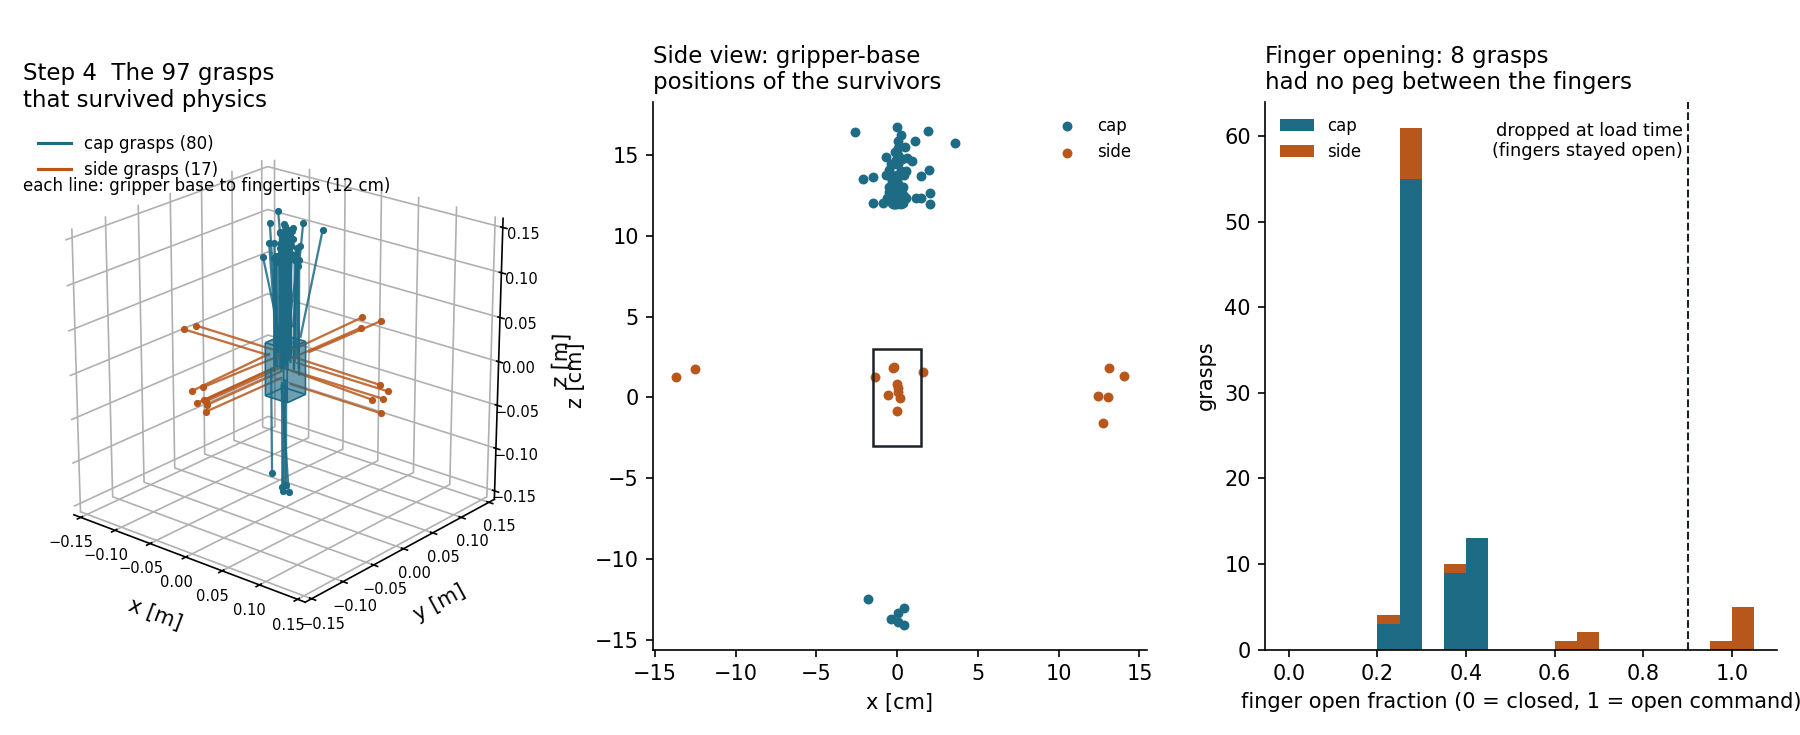
\includegraphics[width=\linewidth]{figures/grasp_f6_survivors.png}
\caption{The 97 recorded grasps: 80 cap grasps (blue) and 17 side grasps (orange). Left and middle: gripper-base positions and approach lines. Right: finger opening at the end of the trial; most stopped at 25 to 45 percent open, which is a 3\,cm peg between fingers that open to 4.45\,cm.}
\label{fig:wsurvivors}
\end{figure}

\subsection{Reset States}
The reset-state generator combines these two files with a full robot and a table. The remainder of these notes is about it.

%==============================================================================
\section{The Recording Environment}
\label{sec:env}

Reset states are recorded by an ordinary Isaac Lab~\cite{mittal2023orbit} manager-based environment that has no observations and no rewards. It has a scene, a set of reset events, a set of termination terms, and a recorder. The script that drives it is \path{scripts_v2/tools/record_reset_states.py}. Each family is a separate registered task, for example \code{OmniReset-G1dDex1-ObjectRestingEEGrasped-v0}.

\paragraph{The scene.}
The scene holds the robot, the insertive object, the receptive object, a table, and a ground plane. The insertive object is a dynamic rigid body with a mass of one gram, so that it does not drag the arm down while held. The receptive object is kinematic, so it never moves. Friction on every body is fixed at a low value by a start-up event. For the G1-D the table is a plain block with the Vention table's footprint and top height.

\paragraph{Timing.}
Physics runs at $120$\,Hz and the environment steps every twelve physics steps, so the control rate is $10$\,Hz. The episode length is two seconds. One recording attempt therefore lasts
\begin{equation}
  N_{\text{steps}} = \frac{T_{\text{episode}}}{\Delta t\, d} = \frac{2.0\ \text{s}}{(1/120\ \text{s})\times 12} = 20\ \text{control steps} = 240\ \text{physics steps}.
\end{equation}

\paragraph{Reset events, by family.}
When an environment resets, its event terms run in declaration order. Every family first restores the scene to its default and places the receptive object at a random pose on the table within a small yaw range. What happens next depends on the family (Table~\ref{tab:events}). Notice that family~2 loads family~1's file through the same \code{MultiResetManager} that training uses. The dependency is literal: if family~1 contains a peg that rolled off the table, family~2 will attempt grasps on the floor.

\begin{table}[t]
\centering
\caption{What the reset events do in each family. ``IK'' is the iterative inverse-kinematics placement of Section~\ref{sec:place}.}
\label{tab:events}
\small
\begin{tabular}{@{}p{3.1cm}p{4.4cm}p{5.4cm}@{}}
\toprule
Family & Insertive object & End effector and fingers\\
\midrule
1 Anywhere / EE anywhere & Uniform pose above the table, up to $25$\,cm high, any orientation & IK to a uniform pose in the workspace, pointing roughly down. Fingers follow the gripper command, drawn at random to be open or closed.\\
2 Resting / EE grasped & A state sampled from the \emph{family~1} file, so the object is already resting as physics left it & IK to a sampled grasp on the object, perturbed by up to $2$\,cm and $11^\circ$. Fingers written to the recorded grasp positions.\\
3 Anywhere / EE grasped & Uniform pose above the table, as in family~1 & IK to a sampled grasp on the object, no perturbation. Fingers written to the recorded grasp positions.\\
4 Partially assembled / EE grasped & A relative pose sampled from the partial-assembly file, composed with the hole's pose & IK to a sampled grasp, perturbed by up to $1$\,cm and $6^\circ$. Fingers written to the recorded grasp positions.\\
\bottomrule
\end{tabular}
\end{table}

\paragraph{Termination terms.}
Four terms can end an episode. Their names matter, because the recorder looks for a term called \code{success}.
\begin{description}[leftmargin=*, itemsep=2pt]
  \item[\code{time\_out}] ends the episode after twenty steps. Nothing is saved.
  \item[\code{abnormal\_robot}] ends the episode at once if any joint moves faster than twice its velocity limit, which indicates a solver explosion.
  \item[\code{grasp\_placement\_failed}] applies to the grasped families only. It ends the episode at the first step if the IK placement ended more than $1$\,cm or $10^\circ$ from the sampled grasp pose. Such an attempt can never pass the success test, so holding it for two seconds would only cost time. Families without a grasp event never trigger it.
  \item[\code{success}] is evaluated every step but can only be true on the final step, as Section~\ref{sec:test} explains. When it is true the episode is exported.
\end{description}

\paragraph{Actions during the hold.}
The arm action is zero. The operational-space controller therefore holds the end effector where the reset placed it, with its own stiffness and damping. The gripper action is the last element of the action vector. For any family whose name contains \code{EEGrasped} it is held at $-1$, the close command, for the whole run. For the other families it is drawn at random from $\{-1,+1\}$ per environment and redrawn whenever that environment resets, so the first family contains both open and closed hands.

\paragraph{The recorder.}
The recorder manager is configured with a single term that fires just before an environment resets. The term calls the scene's state query for the environments that are about to reset and returns it under the key \code{initial\_state}. The export mode is ``succeeded only''. Isaac Lab's reset routine reads the \code{success} termination term for the resetting environments, marks their episodes accordingly, and the manager appends only the marked ones to the file. A reset state is therefore the scene \emph{as it stands after the two-second hold}, not as the events placed it. It is already settled.

%==============================================================================
\section{One Episode, Step by Step}
\label{sec:episode}

\begin{figure}[t]
\centering
\resizebox{\linewidth}{!}{%
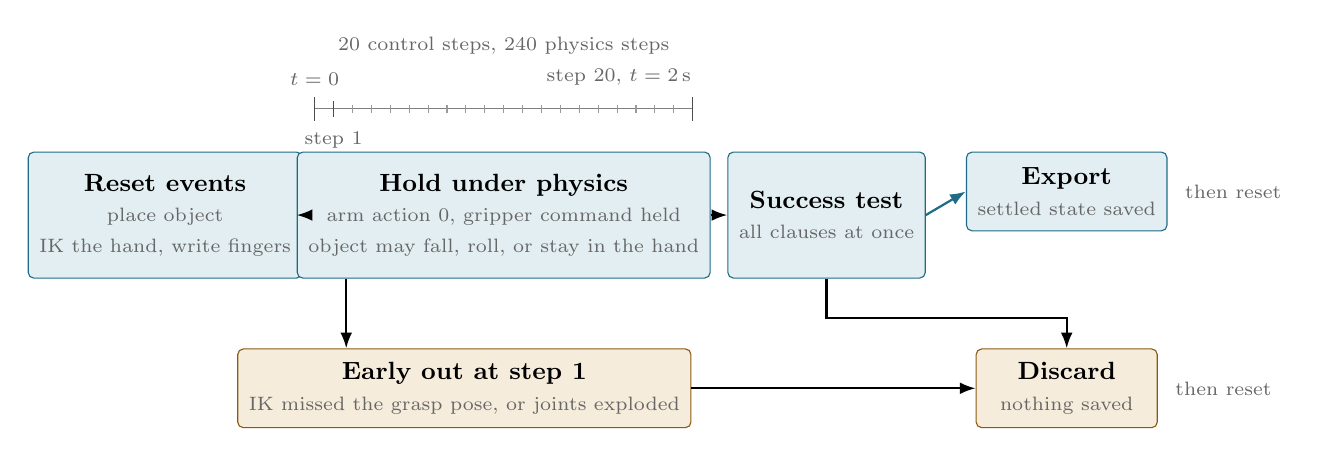
\begin{tikzpicture}[x=1cm, y=1cm,
  phase/.style={draw=accent, fill=accentsoft, rounded corners=2pt, align=center, inner sep=4pt, font=\small},
  good/.style={draw=accent, fill=accentsoft, rounded corners=2pt, align=center, inner sep=4pt, font=\small},
  bad/.style={draw=warn, fill=warnsoft, rounded corners=2pt, align=center, inner sep=4pt, font=\small}]
  % main flow
  \node[phase, minimum width=26mm, minimum height=16mm] (reset) at (1.3,0.8) {\textbf{Reset events}\\ \subl{place object}\\ \subl{IK the hand, write fingers}};
  \node[phase, minimum width=48mm, minimum height=16mm] (hold) at (5.6,0.8) {\textbf{Hold under physics}\\ \subl{arm action $0$, gripper command held}\\ \subl{object may fall, roll, or stay in the hand}};
  \node[phase, minimum width=22mm, minimum height=16mm] (test) at (9.7,0.8) {\textbf{Success test}\\ \subl{all clauses at once}};
  \node[good, minimum width=23mm, minimum height=10mm] (export) at (12.75,1.1) {\textbf{Export}\\ \subl{settled state saved}};
  \node[bad, minimum width=23mm, minimum height=10mm] (discard) at (12.75,-1.4) {\textbf{Discard}\\ \subl{nothing saved}};
  \node[bad, minimum width=38mm, minimum height=10mm] (early) at (5.1,-1.4) {\textbf{Early out at step 1}\\ \subl{IK missed the grasp pose, or joints exploded}};
  \draw[arr] (reset) -- (hold);
  \draw[arr] (hold) -- (test);
  \draw[karr] (test.east) -- (export.west);
  \draw[arr] (test.south) -- ++(0,-0.5) -| (discard.north);
  \draw[arr] ([xshift=-20mm]hold.south) -- ([xshift=-20mm]hold.south |- early.north);
  \draw[arr] (early.east) -- (discard.west);
  \node[sub, anchor=west] at ([xshift=1mm]export.east) {then reset};
  \node[sub, anchor=west] at ([xshift=1mm]discard.east) {then reset};
  % time axis over the hold phase
  \draw[black!50] (3.2,2.15) -- (8.0,2.15);
  \foreach \x in {3.2,3.44,...,8.0} {\draw[black!40] (\x,2.1) -- (\x,2.2);}
  \draw[black!70] (3.2,2.0) -- (3.2,2.3); \node[sub, anchor=south] at (3.2,2.32) {$t=0$};
  \draw[black!70] (3.44,2.05) -- (3.44,2.25); \node[sub, anchor=north] at (3.44,1.98) {step 1};
  \draw[black!70] (8.0,2.0) -- (8.0,2.3); \node[sub, anchor=south east] at (8.1,2.32) {step 20, $t=2$\,s};
  \node[sub, anchor=south] at (5.6,2.72) {20 control steps, 240 physics steps};
\end{tikzpicture}}
\caption{One recording attempt in one environment. The hold lasts twenty control steps, and the success test runs only at the last one. A placement that missed the grasp pose, or a solver blow-up, leaves at step one without waiting. Thousands of these attempts run in parallel, and the script counts exported episodes until it reaches the requested number.}
\label{fig:timeline}
\end{figure}

Follow one environment through Figure~\ref{fig:timeline}.
\begin{enumerate}[leftmargin=*, itemsep=2pt]
  \item \textbf{Reset.} The scene returns to its defaults. The receptive object is placed. The insertive object is placed by the family's rule. For a grasped family, a grasp is drawn, the end-effector target is composed, the iterative IK writes the arm joints, and the finger joints are written to the recorded values. The success term records the end-effector position and each object's position as the reference for the deviation test, and the stability counter is zeroed.
  \item \textbf{Step 1.} Physics runs twelve substeps. If the IK residual from the reset was too large, or any joint velocity is abnormal, the episode ends here. Otherwise the hold begins.
  \item \textbf{Steps 2 through 19.} The arm holds. The gripper tracks its command. Whatever is not physically consistent falls, slides, or settles. On every step the success term checks whether all bodies are nearly at rest and increments a counter, resetting it to zero whenever anything moves. At least five consecutive quiet steps are required at the end.
  \item \textbf{Step 20.} The time-out flag becomes true, and only now can the success term return true. Every clause of Section~\ref{sec:test} is evaluated on the state as it stands.
  \item \textbf{Export.} If successful, the recorder copies the environment's full state into the dataset file. In both cases the environment resets and the cycle restarts.
\end{enumerate}

The script tracks the recorder's count of exported episodes and stops when it reaches \code{--num\_reset\_states}. Because attempts are cheap and failures are common, the yield is best thought of as a rate. If an attempt succeeds with probability $p$ and $E$ environments run in parallel, the expected number of control steps needed to collect $n$ states is
\begin{equation}
  \E[\text{steps}] \approx \frac{n}{p\,E}\times 20 .
  \label{eq:cost}
\end{equation}
At the smoke-test scale used in the repository, $256$ environments and $8$ states per family, the grasped families succeed in between $0.01$ and $0.06$ percent of attempts and take between two and seven minutes. The first family succeeds far more often because it asks for much less.

%==============================================================================
\section{Placing the Hand on a Grasp}
\label{sec:place}

The grasped families reuse a grasp that was recorded with a bare gripper. The event \code{reset\_end\_effector\_from\_grasp\_dataset} must turn that relative pose into joint angles for the whole arm. The computation has three parts.

\paragraph{Composing the target.}
Write $\Tf{A}{B}$ for the pose of frame $B$ expressed in frame $A$. The dataset stores the gripper in the object frame, $\Tf{\obj}{\grip}$, and the object has just been placed at $\Tf{\w}{\obj}$ in the world. The desired gripper pose in the world is therefore
\begin{equation}
  \Tf{\w}{\grip} = \Tf{\w}{\obj}\,\Tf{\obj}{\grip}.
\end{equation}
The IK solver works in the robot's base frame, so the target is expressed there, and an optional perturbation $T_\delta$, drawn uniformly from the family's \code{pose\_range\_b}, is applied on the right, that is, in the gripper's own frame:
\begin{equation}
  \Tf{\base}{\tgt} = \big(\Tf{\w}{\base}\big)^{-1}\,\Tf{\w}{\grip}\,T_\delta .
  \label{eq:target}
\end{equation}
The event also stores the target back in the object frame, $\Tf{\obj}{\tgt}=(\Tf{\w}{\obj})^{-1}\,\Tf{\w}{\base}\,\Tf{\base}{\tgt}$, perturbation included. Section~\ref{sec:test} compares the end effector against this quantity after the hold, which is how the test knows that the hand is on the object rather than merely near it.

\paragraph{Iterating the inverse kinematics.}
Isaac Lab's differential IK with damped least squares~\cite{buss2004introduction,lynch2017modern} gives, from the current joint vector $\bm q_k$ and the pose error, a joint target $\bm q^{*}_k$. Rather than jumping to it, the event takes a quarter step, clamps to the joint limits, and writes the result straight into the simulation without stepping physics:
\begin{equation}
  \bm q_{k+1} = \clamp\!\Big(\bm q_k + \tfrac14\,(\bm q^{*}_k-\bm q_k),\ \bm q_{\min},\ \bm q_{\max}\Big), \qquad k=0,\dots,24 .
  \label{eq:ik}
\end{equation}
Twenty-five iterations at a quarter step each drive the pose error down by a factor of roughly $0.75^{25}\approx10^{-3}$ whenever the target is reachable. Writing the joint state, rather than commanding it, means that the forward kinematics are refreshed on the next read, so each iteration sees the new pose. The clamp is essential. Without it the wrist roll and yaw were routinely written several radians beyond their limits; PhysX snapped them back on the first physics step, and the hand was thrown away from the object it had been placed on.

\paragraph{Recording the residual.}
After the last iteration the event measures how far the end effector ended from the target, in position and in angle, and stores the two numbers per environment. The \code{grasp\_placement\_failed} termination reads them and discards any attempt beyond $1$\,cm or $10^\circ$ at step one. Every twentieth call the event prints the fraction of environments that reached the target together with the median and ninetieth-percentile errors, which is the quickest way to see whether a layout is reachable at all. Finally the finger joints are written to the positions recorded in the grasp. Grasps whose fingers were recorded nearly fully open, more than ninety percent of the way from the close command to the open command, are dropped when the file is loaded, because such a ``grasp'' was an object lying across open fingers.

\paragraph{Reach is a property of the layout.}
An offline probe of the G1-D with the Dex1 gripper found that only about $28\%$ of resting-peg and grasp pairs are reachable within $1$\,cm and $10^\circ$, and that neither more iterations nor other random seeds change that number. Reachability falls sharply beyond $36$\,cm from the robot, because the grasp centre of a top-down Dex1 grasp sits $16$\,cm below the wrist. The remedy is to move the robot closer to the table or to narrow the spawn ranges in the layout file, not to tune the IK.

%==============================================================================
\section{The Success Test, Clause by Clause}
\label{sec:test}

The term \code{check\_reset\_state\_success} returns the conjunction of several boolean clauses. A state is saved only if every clause holds at the final step. Table~\ref{tab:clauses} lists them in the order the code evaluates them, with the values used for the G1-D peg task.

\begin{table}[t]
\centering
\caption{The clauses of the success test. Clauses marked (G) apply to the grasped families only; the last applies to family~4 only.}
\label{tab:clauses}
\small
\begin{tabular}{@{}p{2.4cm}p{6.0cm}p{4.5cm}@{}}
\toprule
Clause & Condition & Why it is there\\
\midrule
Time out & Step counter has reached $20$ & The state must have survived the full hold.\\
No abnormal gripper & No joint faster than twice its velocity limit & Rejects solver blow-ups.\\
Approach points down & The gripper approach axis, rotated into the world, has $z<-0.5$, i.e.\ within $60^\circ$ of straight down & Keeps hand orientations in the range a top-down insertion policy will see.\\
Stable & Five consecutive steps with robot joint speeds summing below $5$\,rad/s and each object's linear speed below $0.1$\,m/s and angular speed below $1$\,rad/s & The scene has settled; starting mid-fall would be unfair.\\
Small deviation & End effector moved less than $10$\,cm since reset; each object moved less than the family's limit: unbounded for family~1, $1$\,cm for~2, $5$\,cm for~3, $2.5$\,cm for~4 & The state must be close to what was asked for. A grasped peg that slid $5$\,cm was not really grasped.\\
Above the table & Every body above \code{pos\_z\_threshold}, for the G1-D $2$\,cm below the table top & A peg that rolled off the edge is not a usable start.\\
Collision free & Three point-cloud distance checks pass & No interpenetration between robot and objects, or between the objects.\\
Fingers blocked (G) & Every finger's open fraction lies strictly between $0.08$ and $0.9$ & Something is between the fingers, and the hand is not simply open.\\
Object near the hand (G) & Object origin within $20$\,cm of the end-effector body & Coarse sanity check.\\
At the grasp pose (G) & End effector, in the object frame, within $1.5$\,cm and $15^\circ$ of the target stored at reset & Tells a hand closed on the peg from one closed on the hole, the table edge, or thin air nearby.\\
Assembly match (4) & Half of the environments must be within $1.5$ times the assembly success threshold, the other half must not be & Keeps a balance of ``nearly done'' and ``still jammed'' starts.\\
\bottomrule
\end{tabular}
\end{table}

\paragraph{The open fraction.}
Several clauses need to know how closed a gripper is without knowing its mechanism. The code reads the open and close command dictionaries of the task's binary gripper action and, for each commanded joint with position $\theta$, computes
\begin{equation}
  f_{\text{open}} = \left|\frac{\theta-\theta_{\text{closed}}}{\theta_{\text{open}}-\theta_{\text{closed}}}\right| ,
  \label{eq:open}
\end{equation}
which is zero at the close command and one at the open command. A gripper that closes on nothing reaches $f_{\text{open}}\approx0$; one that closes on a $2$\,cm peg stops partway; one that was never commanded closed sits at $f_{\text{open}}\approx1$. The same quantity, with the roles reversed, is used by the grasp recorder's ``fingers travelled at least ten percent'' clause.

\paragraph{The collision analyzer.}
Interpenetration is measured, not inferred from contacts. At start-up the analyzer samples $1024$ points on the surface of each link of the asset being checked and builds a signed-distance representation of each obstacle from its collision meshes. On every call it transforms the point cloud into each obstacle's frame and queries the signed distance of every point. The clause holds when the smallest distance is at or above a per-pair minimum: half a millimetre of allowed penetration between robot and insertive object, none between robot and receptive object, and one millimetre between the two objects. The small negative allowances absorb solver tolerance in a grasp without accepting a finger inside a peg.

\paragraph{Reading the funnel.}
With the optional \code{collect\_funnel} parameter the term counts, over all environments whose hold just ended, how many passed each clause, and the debug tool prints the table. It is the first thing to look at when a family yields nothing, because it says which clause is doing the rejecting. In the resting family, before the fixes of Section~\ref{sec:failures}, $73\%$ of holds failed the deviation clause alone, and the grasp-pose clause then removed almost everything that remained.

%==============================================================================
\section{Running the Generator}
\label{sec:run}

The generator runs inside the project's Docker image. Locally the wrapper \path{docker/forge/run_local.sh} mounts the working copy and runs any command; the cluster pipeline \path{docker/forge/g1d_pipeline.sh} runs the same commands in its \code{datasets} stage, in the order fixed by Figure~\ref{fig:deps}:

\begin{lstlisting}[language=bash]
# 1. partial assemblies for the object pair
python scripts_v2/tools/record_partial_assemblies.py --task OmniReset-PartialAssemblies-v0 \
    --num_envs 10 --num_trajectories 10 --dataset_dir $DATA_DIR \
    env.scene.insertive_object=peg env.scene.receptive_object=peghole

# 2. grasps on the insertive object with the Dex1 gripper
python scripts_v2/tools/record_grasps.py --task OmniReset-Dex1-GraspSampling-v0 \
    --num_envs 8192 --num_grasps 1000 --dataset_dir $DATA_DIR \
    --gripper_body_name right_dex1_base_link env.scene.object=peg

# 3. the four families, in this order
for RT in ObjectAnywhereEEAnywhere ObjectRestingEEGrasped \
          ObjectAnywhereEEGrasped ObjectPartiallyAssembledEEGrasped; do
  python scripts_v2/tools/record_reset_states.py --task OmniReset-G1dDex1-${RT}-v0 \
      --num_envs 2048 --num_reset_states 10000 --dataset_dir $DATA_DIR \
      env.scene.insertive_object=peg env.scene.receptive_object=peghole
done
\end{lstlisting}

The pipeline's defaults are $2048$ environments and $10\,000$ states per family; the environment variables \code{RESET\_ENVS}, \code{NUM\_RESETS}, \code{GRASP\_ENVS} and \code{NUM\_GRASPS} override them. The stage is cached on the shared disk and skipped when the last family's file already exists, so a regeneration after a code change needs \code{FORCE=1}. The script itself does three things for the user: it sets the seed to \code{None}, so that every run explores different configurations; it infers the family from the task name and derives the pair directory from the two USD paths, so that the output lands where the training environment will look for it; and it fixes the gripper command, closed for any \code{EEGrasped} task and random otherwise.

Three tools look at a finished file. \code{visualize\_reset\_states.py} cycles through states in a window. \code{render\_reset\_states.py} writes one image per state headlessly and, with \code{--settle\_steps 240 --gripper close}, shows the same state after a further two seconds with the task's own controller holding the arm and the gripper commanded closed, which is the fairest picture of what a policy will inherit. \code{debug\_reset\_env.py --funnel --close\_gripper} runs the recording environment and prints the clause-by-clause funnel.

%==============================================================================
\section{What Goes Wrong, and What It Looks Like}
\label{sec:failures}

Each clause of the success test exists because some plausible-looking state passed without it. The following failures were all observed on the G1-D peg task.
\begin{description}[leftmargin=*, itemsep=3pt]
  \item[The hand is closed on the hole, or on the table, and the peg lies nearby.] The older test required only that the fingers be stopped and the peg within $20$\,cm. A hand that closed on the rim of the hole satisfied both. The grasp-pose clause, which compares the end effector with the stored target in the object frame, is the fix.
  \item[An open hand hovers above a partly inserted peg.] The recorder once commanded the gripper closed only for two families by name, and the partially assembled family was not among them. Half of its environments held with open fingers, and an open hand trivially satisfies ``not fully closed''. The recorder now closes for every grasped family, and the test rejects a hand more than ninety percent open.
  \item[The hand jumps away on the first physics step.] IK solutions beyond the joint limits were snapped back by PhysX. Clamping each iterate, Eq.~\eqref{eq:ik}, removed most of the $10$\,cm deviations.
  \item[No grasp fits a peg lying on its side.] With all surface samples biased to the top of the mesh, every grasp approached along the peg's axis. A lying peg then needed a horizontal approach, which the ``points down'' clause rejects. Mixing in uniform surface samples produced grasps across the diameter.
  \item[A peg on the floor.] Family~1's original height threshold was inherited from the UR5e, whose mounting plate sits near the origin. For the floor-standing G1-D it had to be raised to just below the table top.
  \item[Everything is slow.] Most grasped attempts are unreachable and were held for the full two seconds. Ending them at step one made recording three to six times faster.
\end{description}

%==============================================================================
\section{Exercises}
\label{sec:exercises}

Solutions are given in Appendix~\ref{app:solutions}.
\begin{enumerate}[leftmargin=*, itemsep=3pt, label=\textbf{E\arabic*.}]
  \item Why can the \code{success} term never be true before the last step, even though it is evaluated every step?
  \item A recorded grasped state is restored at the start of a training episode and the peg immediately falls. Nothing is wrong with the dataset. Explain.
  \item Family~2 yields nothing. The funnel shows almost every attempt failing the deviation clause for the robot. Where do you look first?
  \item Why is the perturbation $T_\delta$ in Eq.~\eqref{eq:target} applied in the gripper frame rather than in the object frame?
  \item Equation~\eqref{eq:cost} says that doubling the number of environments halves the time. When does that stop being true?
\end{enumerate}

%==============================================================================
\section{Limitations}

These notes describe the generator as implemented on the \code{feature/forge-omnireset} branch of the UWLab repository on 27~October 2026 and may drift from later revisions. The thresholds quoted are those of the G1-D peg task; the UR5e configurations share the code but differ in several numbers, most visibly the height threshold. The yields quoted were measured at smoke-test scale and will differ on the cluster. The reachability figure comes from an offline kinematic probe, not from the simulator, and depends on the layout file at the time of writing.

\bibliography{references}

\appendix
\section{Solutions to the Exercises}
\label{app:solutions}
\begin{enumerate}[leftmargin=*, itemsep=3pt, label=\textbf{E\arabic*.}]
  \item Because the time-out flag, which is true only when the step counter has reached the episode length, is one of the conjuncts. Every other clause may hold at step~7, but the conjunction is false until step~20. This guarantees that each saved state has survived the complete hold.
  \item The dataset stores finger \emph{positions}, not finger \emph{commands}. The recorder held the gripper closed, so the fingers pressed on the peg. On restore the positions are the same but no command is active until the policy's first action. If that action opens the gripper, or the controller's default target is the open position, the squeeze disappears and the peg drops. The grasp was valid; the policy has to keep it.
  \item At the IK placement, not at the success test. A robot that moves more than $10$\,cm during a hold with a zero arm action was placed somewhere physics would not accept, most often beyond a joint limit or in collision. Check the IK print-out for the fraction of environments reaching the target, then whether the placement respects joint limits, then whether the layout is within reach at all.
  \item Because the perturbation models imprecision of the hand, such as a grasp a centimetre further along the fingers or rotated slightly about the approach axis. Those are naturally expressed in the gripper's own axes. The same numbers applied in the object frame would mean something different for every grasp orientation.
  \item When the GPU is saturated. Each environment adds physics bodies, contact pairs and a $1024$-point collision cloud per link. Past the point where a single step no longer takes constant time, more environments make each step slower and the gain flattens. The formula also assumes that the success probability is independent of the batch, which holds here because environments do not interact.
\end{enumerate}

\end{document}
